\documentclass[twoside]{book}

% Packages required by doxygen
\usepackage{fixltx2e}
\usepackage{calc}
\usepackage{doxygen}
\usepackage[export]{adjustbox} % also loads graphicx
\usepackage{graphicx}
\usepackage[utf8]{inputenc}
\usepackage{makeidx}
\usepackage{multicol}
\usepackage{multirow}
\PassOptionsToPackage{warn}{textcomp}
\usepackage{textcomp}
\usepackage[nointegrals]{wasysym}
\usepackage[table]{xcolor}

% Font selection
\usepackage[T1]{fontenc}
\usepackage[scaled=.90]{helvet}
\usepackage{courier}
\usepackage{amssymb}
\usepackage{sectsty}
\renewcommand{\familydefault}{\sfdefault}
\allsectionsfont{%
  \fontseries{bc}\selectfont%
  \color{darkgray}%
}
\renewcommand{\DoxyLabelFont}{%
  \fontseries{bc}\selectfont%
  \color{darkgray}%
}
\newcommand{\+}{\discretionary{\mbox{\scriptsize$\hookleftarrow$}}{}{}}

% Page & text layout
\usepackage{geometry}
\geometry{%
  a4paper,%
  top=2.5cm,%
  bottom=2.5cm,%
  left=2.5cm,%
  right=2.5cm%
}
\tolerance=750
\hfuzz=15pt
\hbadness=750
\setlength{\emergencystretch}{15pt}
\setlength{\parindent}{0cm}
\setlength{\parskip}{0.2cm}
\makeatletter
\renewcommand{\paragraph}{%
  \@startsection{paragraph}{4}{0ex}{-1.0ex}{1.0ex}{%
    \normalfont\normalsize\bfseries\SS@parafont%
  }%
}
\renewcommand{\subparagraph}{%
  \@startsection{subparagraph}{5}{0ex}{-1.0ex}{1.0ex}{%
    \normalfont\normalsize\bfseries\SS@subparafont%
  }%
}
\makeatother

% Headers & footers
\usepackage{fancyhdr}
\pagestyle{fancyplain}
\fancyhead[LE]{\fancyplain{}{\bfseries\thepage}}
\fancyhead[CE]{\fancyplain{}{}}
\fancyhead[RE]{\fancyplain{}{\bfseries\leftmark}}
\fancyhead[LO]{\fancyplain{}{\bfseries\rightmark}}
\fancyhead[CO]{\fancyplain{}{}}
\fancyhead[RO]{\fancyplain{}{\bfseries\thepage}}
\fancyfoot[LE]{\fancyplain{}{}}
\fancyfoot[CE]{\fancyplain{}{}}
\fancyfoot[RE]{\fancyplain{}{\bfseries\scriptsize Generated on Thu Nov 19 2015 18\+:23\+:37 for C\+E\+G4166\+\_\+\+R\+T\+S\+\_\+\+Lib by Doxygen }}
\fancyfoot[LO]{\fancyplain{}{\bfseries\scriptsize Generated on Thu Nov 19 2015 18\+:23\+:37 for C\+E\+G4166\+\_\+\+R\+T\+S\+\_\+\+Lib by Doxygen }}
\fancyfoot[CO]{\fancyplain{}{}}
\fancyfoot[RO]{\fancyplain{}{}}
\renewcommand{\footrulewidth}{0.4pt}
\renewcommand{\chaptermark}[1]{%
  \markboth{#1}{}%
}
\renewcommand{\sectionmark}[1]{%
  \markright{\thesection\ #1}%
}

% Indices & bibliography
\usepackage{natbib}
\usepackage[titles]{tocloft}
\setcounter{tocdepth}{3}
\setcounter{secnumdepth}{5}
\makeindex

% Custom commands
\newcommand{\clearemptydoublepage}{%
  \newpage{\pagestyle{empty}\cleardoublepage}%
}


%===== C O N T E N T S =====

\begin{document}

% Titlepage & ToC
\pagenumbering{roman}
\begin{titlepage}
\vspace*{7cm}
\begin{center}%
{\Large C\+E\+G4166\+\_\+\+R\+T\+S\+\_\+\+Lib }\\
\vspace*{1cm}
{\large Generated by Doxygen 1.8.9.1}\\
\vspace*{0.5cm}
{\small Thu Nov 19 2015 18:23:37}\\
\end{center}
\end{titlepage}
\clearemptydoublepage
\tableofcontents
\clearemptydoublepage
\pagenumbering{arabic}

%--- Begin generated contents ---
\chapter{C\+E\+G4166/\+C\+S\+I4141 -\/ Real Time System Library}
\label{index}{\itshape {\bfseries Introduction} {\bfseries to} {\bfseries template}  } \begin{DoxyNote}{Note}
You may use this template to produce your source code, which is documented and coded as per the stipulated standards. This template is produced using Eclipse I\+D\+E and Doxygen document generation tool. You may refer to Documentation and Coding Standards -\/ Guidelines for more details; or you may visit respective official web-\/site. ~\newline
\begin{TabularC}{2}
\hline
\rowcolor{lightgray}{\bf Description }&{\bf Web-\/link/\+Document  }\\\cline{1-2}
Documentation and Coding Standards -\/ Guidelines &documentation\+\_\+and\+\_\+coding\+\_\+standard\+\_\+guidelines.\+pdf \\\cline{1-2}
Doxygen Command Reference &doxygen\+\_\+command\+\_\+reference.\+pdf \\\cline{1-2}
Doxygen Document Generation &\href{http://www.stack.nl/~dimitri/doxygen}{\tt Doxygen} \\\cline{1-2}
G\+N\+U Coding Standards &\href{http://www.gnu.org/prep/standards/standards.html}{\tt G\+N\+U Coding Standards} \\\cline{1-2}
\end{TabularC}

\end{DoxyNote}
\begin{DoxyAttention}{Attention}
Remember to remove and/or replace each section/topic of source file and respective documentation with relevant and applicable information applicable to your project. 
\end{DoxyAttention}
\begin{DoxyWarning}{Warning}
It is recommended and required to read through and understand the concepts from respective guide before attempting to use this template.
\end{DoxyWarning}




\begin{DoxyAuthor}{Author}
provide author details 
\end{DoxyAuthor}
\begin{DoxyDate}{Date}
provide date 
\end{DoxyDate}
\begin{DoxyCopyright}{Copyright}
provide copyright information 
\end{DoxyCopyright}
\begin{DoxyParagraph}{You may provide an overview of the project. Details can be organized in multiple sections and subsection.}
Replace below the section/subsection names and corresponding description/details according to need. 
\end{DoxyParagraph}
\hypertarget{index_section_name_1}{}\section{Section 1 provide section name and description}\label{index_section_name_1}
\begin{DoxyParagraph}{Put your Paragraph describing section}
~\newline

\end{DoxyParagraph}
\hypertarget{index_subsection_name_1_1}{}\subsection{Subsection 1.\+1 provide subsection name and description}\label{index_subsection_name_1_1}
\begin{DoxyParagraph}{(paragraph -\/ 01)}

\end{DoxyParagraph}
\begin{DoxyParagraph}{(paragraph -\/ 02)}
~\newline
~\newline

\end{DoxyParagraph}
\hypertarget{index_section_name_2}{}\section{Section 2 provide section name and description}\label{index_section_name_2}
\begin{DoxyParagraph}{Put your Paragraph describing section}

\end{DoxyParagraph}
\hypertarget{index_subsection_name_2_1}{}\subsection{Subsection 2.\+1 provide subsection name and description}\label{index_subsection_name_2_1}
\begin{DoxyParagraph}{(paragraph -\/ 01)}

\end{DoxyParagraph}
\begin{DoxyParagraph}{(paragraph -\/ 02)}

\end{DoxyParagraph}
\begin{DoxyParagraph}{}

\end{DoxyParagraph}


 
\chapter{Module Index}
\section{Modules}
Here is a list of all modules\+:\begin{DoxyCompactList}
\item \contentsline{section}{U\+S\+A\+R\+T Asynchronous Serial Module Testing}{\pageref{group__testing_u_s_a_r_t_module}}{}
\item \contentsline{section}{U\+S\+A\+R\+T Asynchronous Serial Module Testing}{\pageref{group__test_lib_module}}{}
\end{DoxyCompactList}

\chapter{Data Structure Index}
\section{Data Structures}
Here are the data structures with brief descriptions\+:\begin{DoxyCompactList}
\item\contentsline{section}{{\bf encoder\+\_\+config\+\_\+t} }{\pageref{structencoder__config__t}}{}
\item\contentsline{section}{{\bf motor\+\_\+registers\+\_\+s} }{\pageref{structmotor__registers__s}}{}
\item\contentsline{section}{{\bf tc\+\_\+module\+\_\+registers} }{\pageref{structtc__module__registers}}{}
\item\contentsline{section}{{\bf U\+S\+A\+R\+T\+\_\+\+C\+O\+M\+\_\+\+B\+U\+F} \\*Structure of buffers to support communications with a U\+S\+A\+R\+T }{\pageref{struct_u_s_a_r_t___c_o_m___b_u_f}}{}
\item\contentsline{section}{{\bf U\+S\+A\+R\+T\+\_\+\+R\+E\+G\+I\+S\+T\+E\+R\+S} \\*Structure of pointers to U\+S\+A\+R\+T registers }{\pageref{struct_u_s_a_r_t___r_e_g_i_s_t_e_r_s}}{}
\end{DoxyCompactList}

\chapter{File Index}
\section{File List}
Here is a list of all documented files with brief descriptions\+:\begin{DoxyCompactList}
\item\contentsline{section}{{\bf usart\+Serial.\+c} \\*Module for asynchronous communication with the Atmega2560 U\+S\+A\+R\+T\textquotesingle{}s }{\pageref{usart_serial_8c}}{}
\end{DoxyCompactList}

\chapter{Module Documentation}
\section{U\+S\+A\+R\+T Asynchronous Serial Module}
\label{group__usart_async_module}\index{U\+S\+A\+R\+T Asynchronous Serial Module@{U\+S\+A\+R\+T Asynchronous Serial Module}}
\subsection*{Data Structures}
\begin{DoxyCompactItemize}
\item 
struct {\bf U\+S\+A\+R\+T\+\_\+\+C\+O\+M\+\_\+\+B\+U\+F}
\begin{DoxyCompactList}\small\item\em Structure of buffers to support communications with a U\+S\+A\+R\+T. \end{DoxyCompactList}\item 
struct {\bf U\+S\+A\+R\+T\+\_\+\+R\+E\+G\+I\+S\+T\+E\+R\+S}
\begin{DoxyCompactList}\small\item\em Structure of pointers to U\+S\+A\+R\+T registers. \end{DoxyCompactList}\end{DoxyCompactItemize}
\subsection*{Macros}
\begin{DoxyCompactItemize}
\item 
\#define {\bfseries R\+X\+C\+\_\+\+B\+I\+T}~B\+I\+T7\label{group__usart_async_module_ga2133aeaf30d1d8f6f819d2252dcdbe8c}

\item 
\#define {\bfseries T\+X\+C\+\_\+\+B\+I\+T}~B\+I\+T6\label{group__usart_async_module_ga6baa91108d3c2d172e44bc70956b98d2}

\item 
\#define {\bfseries U\+D\+R\+E\+\_\+\+B\+I\+T}~B\+I\+T5\label{group__usart_async_module_ga774a9a790e2e547044eddf47e931a1f8}

\item 
\#define {\bfseries F\+E\+\_\+\+B\+I\+T}~B\+I\+T4\label{group__usart_async_module_gaaee51057462df51f411e67a131165914}

\item 
\#define {\bfseries D\+O\+R\+\_\+\+B\+I\+T}~B\+I\+T3\label{group__usart_async_module_ga42bba56b7ce519d770f6791da46b3f64}

\item 
\#define {\bfseries U\+P\+E\+\_\+\+B\+I\+T}~B\+I\+T2\label{group__usart_async_module_gaaa081c9d68175cca9b7a57927616baf1}

\item 
\#define {\bfseries U2\+X\+\_\+\+B\+I\+T}~B\+I\+T1\label{group__usart_async_module_gaffd8feb2e774dd114102f1f8be6599aa}

\item 
\#define {\bfseries R\+X\+C\+I\+E\+\_\+\+B\+I\+T}~B\+I\+T7\label{group__usart_async_module_ga4155881309ac7b270c766149bc9a4bbd}

\item 
\#define {\bfseries U\+D\+R\+I\+E\+\_\+\+B\+I\+T}~B\+I\+T5\label{group__usart_async_module_gaf64c1f6cfda10c415407572973d3f71c}

\item 
\#define {\bfseries R\+X\+E\+N\+\_\+\+B\+I\+T}~B\+I\+T4\label{group__usart_async_module_ga906dab704ddcdb3d2d06384a94126c23}

\item 
\#define {\bfseries T\+X\+E\+N\+\_\+\+B\+I\+T}~B\+I\+T3\label{group__usart_async_module_gae3f799c1bacbb79826d19f6f68c9ddde}

\item 
\#define {\bfseries U\+C\+S\+Z1\+\_\+\+B\+I\+T}~B\+I\+T2\label{group__usart_async_module_ga9f7f7ba3dc9cf8409364251f5167589d}

\item 
\#define {\bfseries U\+C\+S\+Z0\+\_\+\+B\+I\+T}~B\+I\+T1\label{group__usart_async_module_gabc8fadc00f40b4574889185ded4f33f2}

\item 
\#define {\bfseries N\+U\+M\+\_\+\+U\+S\+A\+R\+T\+S}~4\label{group__usart_async_module_ga6829feca87a1bc576152b06505b91617}

\end{DoxyCompactItemize}
\subsection*{Enumerations}
\begin{DoxyCompactItemize}
\item 
enum {\bf U\+S\+A\+R\+T\+\_\+\+S\+T\+A\+T\+E} \{ {\bf V\+A\+C\+A\+N\+T}, 
{\bf E\+N\+G\+A\+G\+E\+D}
 \}
\begin{DoxyCompactList}\small\item\em Defines the state of the U\+S\+A\+R\+T. \end{DoxyCompactList}\end{DoxyCompactItemize}
\subsection*{Functions}
\begin{DoxyCompactItemize}
\item 
int8\+\_\+t {\bf usart\+Check\+Rx\+Complete} (U\+S\+A\+R\+T\+\_\+\+I\+D usart\+Id)
\begin{DoxyCompactList}\small\item\em Check if reception is complete. The function returns the status of the R\+X\+C bit of the U\+S\+A\+R\+T. When set, the bit indicates that data can be read from the U\+S\+A\+R\+T. \end{DoxyCompactList}\item 
int8\+\_\+t {\bf usart\+Check\+Tx\+Ready} (U\+S\+A\+R\+T\+\_\+\+I\+D usart\+Id)
\begin{DoxyCompactList}\small\item\em Check if transmission is complete. The function returns the status of the U\+D\+R\+E bit of the U\+S\+A\+R\+T. When set, the bit indicates that data can be written to the U\+S\+A\+R\+T. \end{DoxyCompactList}\item 
void {\bfseries usart\+\_\+fprintf\+\_\+arg} (U\+S\+A\+R\+T\+\_\+\+I\+D usart\+Id, const char $\ast$format, va\+\_\+list ap)\label{group__usart_async_module_gad3cf1cbb614711dcb8b73f7b7066cc24}

\item 
void {\bfseries usart\+\_\+fprintf\+\_\+\+P\+\_\+arg} (U\+S\+A\+R\+T\+\_\+\+I\+D usart\+Id, P\+G\+M\+\_\+\+P format, va\+\_\+list arg)\label{group__usart_async_module_ga8b9e6d432ec75ce20fd8225d02cd8340}

\item 
void {\bfseries usart\+\_\+xfprintf\+\_\+arg} (U\+S\+A\+R\+T\+\_\+\+I\+D usart\+Id, const char $\ast$format, va\+\_\+list arg)\label{group__usart_async_module_ga7f6efaab6a3c0a43d34bcce2f45a9062}

\item 
void {\bfseries usart\+\_\+xfprintf\+\_\+\+P\+\_\+arg} (U\+S\+A\+R\+T\+\_\+\+I\+D usart\+Id, P\+G\+M\+\_\+\+P format, va\+\_\+list arg)\label{group__usart_async_module_ga33e17cf0120f57e061a736a8eeb93fce}

\item 
void {\bf xmit\+Interrupt\+\_\+\+On} (U\+S\+A\+R\+T\+\_\+\+I\+D)
\item 
void {\bf xmit\+Interrupt\+\_\+\+Off} (U\+S\+A\+R\+T\+\_\+\+I\+D)
\item 
void {\bf usart\+\_\+rx\+\_\+isr} (U\+S\+A\+R\+T\+\_\+\+I\+D)
\item 
void {\bf usart\+\_\+tx\+\_\+isr} (U\+S\+A\+R\+T\+\_\+\+I\+D)
\item 
U\+S\+A\+R\+T\+\_\+\+I\+D {\bf usart\+Open} (U\+S\+A\+R\+T\+\_\+\+I\+D usart\+Id, uint32\+\_\+t ul\+Wanted\+Baud, uint16\+\_\+t ux\+Tx\+Queue\+Length, uint16\+\_\+t ux\+Rx\+Queue\+Length)
\begin{DoxyCompactList}\small\item\em Open a connection on a U\+S\+A\+R\+T. \end{DoxyCompactList}\item 
void {\bf set\+Default\+U\+S\+A\+R\+T} (U\+S\+A\+R\+T\+\_\+\+I\+D usart\+Id)
\begin{DoxyCompactList}\small\item\em Update default U\+S\+A\+R\+T. \end{DoxyCompactList}\item 
void {\bf usart\+Close} (U\+S\+A\+R\+T\+\_\+\+I\+D usart\+Id)
\begin{DoxyCompactList}\small\item\em Close a connection on a U\+S\+A\+R\+T. \end{DoxyCompactList}\item 
void {\bf usart\+\_\+printf} (const char $\ast$format,...)
\begin{DoxyCompactList}\small\item\em Standard printf function. \end{DoxyCompactList}\item 
void {\bf usart\+\_\+printf\+\_\+\+P} (P\+G\+M\+\_\+\+P format,...)
\begin{DoxyCompactList}\small\item\em Standard printf function that uses a formating string stored in memory. \end{DoxyCompactList}\item 
void {\bf usart\+\_\+print} (uint8\+\_\+t $\ast$str)
\begin{DoxyCompactList}\small\item\em Print string on default U\+S\+A\+R\+T. \end{DoxyCompactList}\item 
void {\bf usart\+\_\+print\+\_\+\+P} (P\+G\+M\+\_\+\+P str)
\begin{DoxyCompactList}\small\item\em Print string stored in program memory on default U\+S\+A\+R\+T. \end{DoxyCompactList}\item 
void {\bf usart\+\_\+fprintf} (int usartid, const char $\ast$format,...)
\begin{DoxyCompactList}\small\item\em Standard printf for specified U\+S\+A\+R\+T. \end{DoxyCompactList}\item 
void {\bf usart\+\_\+fprintf\+\_\+\+P} (int usart\+Id, P\+G\+M\+\_\+\+P format,...)
\begin{DoxyCompactList}\small\item\em Standard printf function for specific U\+S\+A\+R\+T with formating string in program memory. \end{DoxyCompactList}\item 
void {\bf usart\+\_\+fprint} (U\+S\+A\+R\+T\+\_\+\+I\+D usart\+Id, uint8\+\_\+t $\ast$str)
\begin{DoxyCompactList}\small\item\em Print string to specific U\+S\+A\+R\+T. \end{DoxyCompactList}\item 
void {\bf usart\+\_\+fprint\+\_\+\+P} (U\+S\+A\+R\+T\+\_\+\+I\+D usart\+Id, P\+G\+M\+\_\+\+P str)
\begin{DoxyCompactList}\small\item\em Print a string stored in program memory to specific U\+S\+A\+R\+T. \end{DoxyCompactList}\item 
void {\bf usart\+Write} (U\+S\+A\+R\+T\+\_\+\+I\+D usart\+Id, int8\+\_\+t data\+Out)
\begin{DoxyCompactList}\small\item\em Low level write function (single character). Will delay until usart is ready to accept the 8 bit data. \end{DoxyCompactList}\item 
int8\+\_\+t {\bf usart\+Read} (U\+S\+A\+R\+T\+\_\+\+I\+D usart\+Id)
\begin{DoxyCompactList}\small\item\em Low level read function (single character). Delays until data available from the U\+S\+A\+R\+T. Will check for reception errors. \end{DoxyCompactList}\item 
void {\bf usart\+\_\+xprintf} (const char $\ast$format,...)
\begin{DoxyCompactList}\small\item\em Standard printf (interrupt driven) to default U\+S\+A\+R\+T. \end{DoxyCompactList}\item 
void {\bf usart\+\_\+xprintf\+\_\+\+P} (P\+G\+M\+\_\+\+P format,...)
\begin{DoxyCompactList}\small\item\em Standard printf (interrupt driven) to default U\+S\+A\+R\+T using formating string stored in program memory. \end{DoxyCompactList}\item 
void {\bf usart\+\_\+xprint} (uint8\+\_\+t $\ast$str)
\begin{DoxyCompactList}\small\item\em Prints a string on the default U\+S\+A\+R\+T (defined by default\+U\+S\+A\+R\+T). \end{DoxyCompactList}\item 
void {\bf usart\+\_\+xprint\+\_\+\+P} (P\+G\+M\+\_\+\+P str)
\begin{DoxyCompactList}\small\item\em Prints a string stored in program memory on the default U\+S\+A\+R\+T (defined by default\+U\+S\+A\+R\+T). \end{DoxyCompactList}\item 
void {\bf usart\+\_\+xfprintf} (int usart\+Id, const char $\ast$format,...)
\begin{DoxyCompactList}\small\item\em Standard printf function for specific U\+S\+A\+R\+T. \end{DoxyCompactList}\item 
void {\bf usart\+\_\+xfprintf\+\_\+\+P} (int usart\+Id, P\+G\+M\+\_\+\+P format,...)
\begin{DoxyCompactList}\small\item\em Standard printf function for specific U\+S\+A\+R\+T that uses a formating string stored in program memory. \end{DoxyCompactList}\item 
void {\bf usart\+\_\+xfprint} (U\+S\+A\+R\+T\+\_\+\+I\+D usart\+Id, uint8\+\_\+t $\ast$str)
\begin{DoxyCompactList}\small\item\em Print string to specific U\+S\+A\+R\+T. \end{DoxyCompactList}\item 
void {\bf usart\+\_\+xfprint\+\_\+\+P} (U\+S\+A\+R\+T\+\_\+\+I\+D usart\+Id, P\+G\+M\+\_\+\+P str)
\begin{DoxyCompactList}\small\item\em Print string stored in program memory to specific U\+S\+A\+R\+T. \end{DoxyCompactList}\item 
void {\bf usart\+\_\+xflush\+Rx} (U\+S\+A\+R\+T\+\_\+\+I\+D usart\+Id)
\begin{DoxyCompactList}\small\item\em Flushes all characters in the receive ring buffer (i.\+e. empties the buffer). \end{DoxyCompactList}\item 
uint16\+\_\+t {\bf usart\+\_\+\+Available\+Char\+Rx} (U\+S\+A\+R\+T\+\_\+\+I\+D usart\+Id)
\begin{DoxyCompactList}\small\item\em Gives number of bytes in reception ring buffer. \end{DoxyCompactList}\item 
U\+Base\+Type\+\_\+t {\bf usart\+\_\+xget\+Char} (U\+S\+A\+R\+T\+\_\+\+I\+D usart\+Id, U\+Base\+Type\+\_\+t $\ast$pc\+Rxed\+Char)
\begin{DoxyCompactList}\small\item\em Get a character from the reception ring buffer. \end{DoxyCompactList}\item 
U\+Base\+Type\+\_\+t {\bf usart\+\_\+xput\+Char} (U\+S\+A\+R\+T\+\_\+\+I\+D usart\+Id, const U\+Base\+Type\+\_\+t c\+Out\+Char)
\begin{DoxyCompactList}\small\item\em Drops a character into the transmit ring buffer. \end{DoxyCompactList}\item 
{\bfseries I\+S\+R} (U\+S\+A\+R\+T0\+\_\+\+R\+X\+\_\+vect)\label{group__usart_async_module_ga084f0a9cf05b1877bd8a71a90dae7ff8}

\item 
{\bfseries I\+S\+R} (U\+S\+A\+R\+T1\+\_\+\+R\+X\+\_\+vect)\label{group__usart_async_module_gae6e8a8009a9ae0c59f25a496d1cf5a84}

\item 
{\bfseries I\+S\+R} (U\+S\+A\+R\+T2\+\_\+\+R\+X\+\_\+vect)\label{group__usart_async_module_ga63a86aad9ba2e355fe6380da553f554e}

\item 
{\bfseries I\+S\+R} (U\+S\+A\+R\+T3\+\_\+\+R\+X\+\_\+vect)\label{group__usart_async_module_ga88e32db0cad75219c51253f5c1052fc0}

\item 
{\bfseries I\+S\+R} (U\+S\+A\+R\+T0\+\_\+\+U\+D\+R\+E\+\_\+vect)\label{group__usart_async_module_ga95e67e677722a53e3ad9f1ffce2e7408}

\item 
{\bfseries I\+S\+R} (U\+S\+A\+R\+T1\+\_\+\+U\+D\+R\+E\+\_\+vect)\label{group__usart_async_module_gad6441110baf548d12ae53fcbed8075c5}

\item 
{\bfseries I\+S\+R} (U\+S\+A\+R\+T2\+\_\+\+U\+D\+R\+E\+\_\+vect)\label{group__usart_async_module_ga6dd0f9b7dad929f4170efd85c67e04ba}

\item 
{\bfseries I\+S\+R} (U\+S\+A\+R\+T3\+\_\+\+U\+D\+R\+E\+\_\+vect)\label{group__usart_async_module_ga965b31b0729ebabd50c26e4557d9609d}

\end{DoxyCompactItemize}
\subsection*{Variables}
\begin{DoxyCompactItemize}
\item 
{\bf U\+S\+A\+R\+T\+\_\+\+R\+E\+G\+I\+S\+T\+E\+R\+S} {\bf usart\+Reg} [$\,$]
\item 
{\bf U\+S\+A\+R\+T\+\_\+\+C\+O\+M\+\_\+\+B\+U\+F} {\bf usart\+Com\+Buf} [N\+U\+M\+\_\+\+U\+S\+A\+R\+T\+S]
\item 
U\+S\+A\+R\+T\+\_\+\+I\+D {\bf default\+U\+S\+A\+R\+T} = U\+S\+A\+R\+T0
\end{DoxyCompactItemize}


\subsection{Detailed Description}


\subsection{Enumeration Type Documentation}
\index{U\+S\+A\+R\+T Asynchronous Serial Module@{U\+S\+A\+R\+T Asynchronous Serial Module}!U\+S\+A\+R\+T\+\_\+\+S\+T\+A\+T\+E@{U\+S\+A\+R\+T\+\_\+\+S\+T\+A\+T\+E}}
\index{U\+S\+A\+R\+T\+\_\+\+S\+T\+A\+T\+E@{U\+S\+A\+R\+T\+\_\+\+S\+T\+A\+T\+E}!U\+S\+A\+R\+T Asynchronous Serial Module@{U\+S\+A\+R\+T Asynchronous Serial Module}}
\subsubsection[{U\+S\+A\+R\+T\+\_\+\+S\+T\+A\+T\+E}]{\setlength{\rightskip}{0pt plus 5cm}enum {\bf U\+S\+A\+R\+T\+\_\+\+S\+T\+A\+T\+E}}\label{group__usart_async_module_gab7cdec2c3d93593769da070a66249537}


Defines the state of the U\+S\+A\+R\+T. 

\begin{Desc}
\item[Enumerator]\par
\begin{description}
\index{V\+A\+C\+A\+N\+T@{V\+A\+C\+A\+N\+T}!U\+S\+A\+R\+T Asynchronous Serial Module@{U\+S\+A\+R\+T Asynchronous Serial Module}}\index{U\+S\+A\+R\+T Asynchronous Serial Module@{U\+S\+A\+R\+T Asynchronous Serial Module}!V\+A\+C\+A\+N\+T@{V\+A\+C\+A\+N\+T}}\item[{\em 
V\+A\+C\+A\+N\+T\label{group__usart_async_module_ggab7cdec2c3d93593769da070a66249537a10956a5edaf1667eeca04db9a23a9264}
}]U\+S\+A\+R\+T is available for access. \index{E\+N\+G\+A\+G\+E\+D@{E\+N\+G\+A\+G\+E\+D}!U\+S\+A\+R\+T Asynchronous Serial Module@{U\+S\+A\+R\+T Asynchronous Serial Module}}\index{U\+S\+A\+R\+T Asynchronous Serial Module@{U\+S\+A\+R\+T Asynchronous Serial Module}!E\+N\+G\+A\+G\+E\+D@{E\+N\+G\+A\+G\+E\+D}}\item[{\em 
E\+N\+G\+A\+G\+E\+D\label{group__usart_async_module_ggab7cdec2c3d93593769da070a66249537a376d84b562e172773b813085b438da29}
}]U\+S\+A\+R\+T is engaged by another task. \end{description}
\end{Desc}


\subsection{Function Documentation}
\index{U\+S\+A\+R\+T Asynchronous Serial Module@{U\+S\+A\+R\+T Asynchronous Serial Module}!set\+Default\+U\+S\+A\+R\+T@{set\+Default\+U\+S\+A\+R\+T}}
\index{set\+Default\+U\+S\+A\+R\+T@{set\+Default\+U\+S\+A\+R\+T}!U\+S\+A\+R\+T Asynchronous Serial Module@{U\+S\+A\+R\+T Asynchronous Serial Module}}
\subsubsection[{set\+Default\+U\+S\+A\+R\+T}]{\setlength{\rightskip}{0pt plus 5cm}void set\+Default\+U\+S\+A\+R\+T (
\begin{DoxyParamCaption}
\item[{U\+S\+A\+R\+T\+\_\+\+I\+D}]{usart\+Id}
\end{DoxyParamCaption}
)}\label{group__usart_async_module_gaa679900a334c7873eb71c86fe52cbf40}


Update default U\+S\+A\+R\+T. 

The usart must be initilased with usart\+Open to be used as the default U\+S\+A\+R\+T. 
\begin{DoxyParams}{Parameters}
{\em usart\+Id} & -\/ Usart Identifier. \\
\hline
\end{DoxyParams}
\index{U\+S\+A\+R\+T Asynchronous Serial Module@{U\+S\+A\+R\+T Asynchronous Serial Module}!usart\+\_\+\+Available\+Char\+Rx@{usart\+\_\+\+Available\+Char\+Rx}}
\index{usart\+\_\+\+Available\+Char\+Rx@{usart\+\_\+\+Available\+Char\+Rx}!U\+S\+A\+R\+T Asynchronous Serial Module@{U\+S\+A\+R\+T Asynchronous Serial Module}}
\subsubsection[{usart\+\_\+\+Available\+Char\+Rx}]{\setlength{\rightskip}{0pt plus 5cm}uint16\+\_\+t usart\+\_\+\+Available\+Char\+Rx (
\begin{DoxyParamCaption}
\item[{U\+S\+A\+R\+T\+\_\+\+I\+D}]{usart\+Id}
\end{DoxyParamCaption}
)}\label{group__usart_async_module_gae7ed1c85cf0d965f00c8b8b1adc87621}


Gives number of bytes in reception ring buffer. 

This function can be used to check the number of available characters in the reception ring buffer. Returns 0 if no characters are available in the ring buffer. 
\begin{DoxyParams}{Parameters}
{\em usart\+Id} & -\/ U\+S\+A\+R\+T identifier \\
\hline
\end{DoxyParams}
\begin{DoxyReturn}{Returns}
Number of available characters in the reception ring buffer. Returns 0 of no characters are available. 
\end{DoxyReturn}
\index{U\+S\+A\+R\+T Asynchronous Serial Module@{U\+S\+A\+R\+T Asynchronous Serial Module}!usart\+\_\+fprint@{usart\+\_\+fprint}}
\index{usart\+\_\+fprint@{usart\+\_\+fprint}!U\+S\+A\+R\+T Asynchronous Serial Module@{U\+S\+A\+R\+T Asynchronous Serial Module}}
\subsubsection[{usart\+\_\+fprint}]{\setlength{\rightskip}{0pt plus 5cm}void usart\+\_\+fprint (
\begin{DoxyParamCaption}
\item[{U\+S\+A\+R\+T\+\_\+\+I\+D}]{usart\+Id, }
\item[{uint8\+\_\+t $\ast$}]{str}
\end{DoxyParamCaption}
)}\label{group__usart_async_module_ga5598cc3783a39c313bc27baa10cf9952}


Print string to specific U\+S\+A\+R\+T. 

Transmits a given string to the U\+S\+A\+R\+T. 
\begin{DoxyParams}{Parameters}
{\em usart\+Id} & -\/ U\+S\+A\+R\+T identifier \\
\hline
{\em str} & -\/ String to transmit via the U\+S\+A\+R\+T. \\
\hline
\end{DoxyParams}


Here is the call graph for this function\+:\nopagebreak
\begin{figure}[H]
\begin{center}
\leavevmode
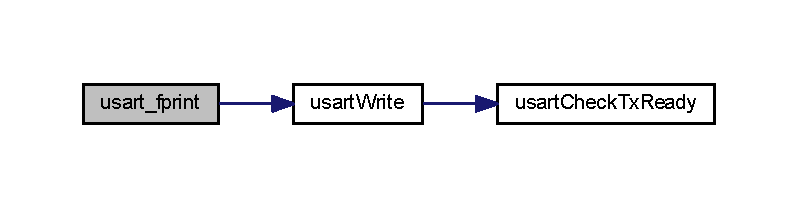
\includegraphics[width=350pt]{group__usart_async_module_ga5598cc3783a39c313bc27baa10cf9952_cgraph}
\end{center}
\end{figure}


\index{U\+S\+A\+R\+T Asynchronous Serial Module@{U\+S\+A\+R\+T Asynchronous Serial Module}!usart\+\_\+fprint\+\_\+\+P@{usart\+\_\+fprint\+\_\+\+P}}
\index{usart\+\_\+fprint\+\_\+\+P@{usart\+\_\+fprint\+\_\+\+P}!U\+S\+A\+R\+T Asynchronous Serial Module@{U\+S\+A\+R\+T Asynchronous Serial Module}}
\subsubsection[{usart\+\_\+fprint\+\_\+\+P}]{\setlength{\rightskip}{0pt plus 5cm}void usart\+\_\+fprint\+\_\+\+P (
\begin{DoxyParamCaption}
\item[{U\+S\+A\+R\+T\+\_\+\+I\+D}]{usart\+Id, }
\item[{P\+G\+M\+\_\+\+P}]{str}
\end{DoxyParamCaption}
)}\label{group__usart_async_module_gaa376b136593fb6bc0e5e9f7b35473f14}


Print a string stored in program memory to specific U\+S\+A\+R\+T. 

Prints a string stored in the program memory to the U\+S\+A\+R\+T identified by usart\+Id. Special functions are required to access the string stored in program memory. 
\begin{DoxyParams}{Parameters}
{\em usart\+Id} & -\/ U\+S\+A\+R\+T identifier. \\
\hline
{\em str} & -\/ String for transmitting over U\+S\+A\+R\+T. \\
\hline
\end{DoxyParams}


Here is the call graph for this function\+:\nopagebreak
\begin{figure}[H]
\begin{center}
\leavevmode
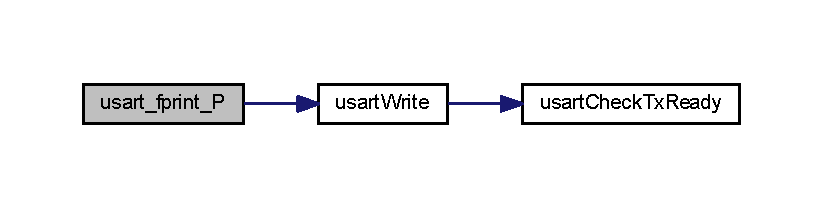
\includegraphics[width=350pt]{group__usart_async_module_gaa376b136593fb6bc0e5e9f7b35473f14_cgraph}
\end{center}
\end{figure}


\index{U\+S\+A\+R\+T Asynchronous Serial Module@{U\+S\+A\+R\+T Asynchronous Serial Module}!usart\+\_\+fprintf@{usart\+\_\+fprintf}}
\index{usart\+\_\+fprintf@{usart\+\_\+fprintf}!U\+S\+A\+R\+T Asynchronous Serial Module@{U\+S\+A\+R\+T Asynchronous Serial Module}}
\subsubsection[{usart\+\_\+fprintf}]{\setlength{\rightskip}{0pt plus 5cm}void usart\+\_\+fprintf (
\begin{DoxyParamCaption}
\item[{int}]{usartid, }
\item[{const char $\ast$}]{format, }
\item[{}]{...}
\end{DoxyParamCaption}
)}\label{group__usart_async_module_ga7429cdd4ac36c036e982817d6750ed34}


Standard printf for specified U\+S\+A\+R\+T. 

This function has a variable list and uses the variable list feature of C (see documentation on stdarg). The function uses vsnprintf function for formating the string to output in the work\+Buffer before transmission. This function calls usart\+\_\+print to send the contents of the work buffer to the U\+S\+A\+R\+T. 
\begin{DoxyParams}{Parameters}
{\em usart\+Id} & -\/ U\+S\+A\+R\+T identifier -\/ note that var\+\_\+list, va\+\_\+start, etc does not work when using U\+S\+E\+R\+I\+D enumerated types. must be an int. \\
\hline
{\em format} & -\/ Formating string. \\
\hline
\end{DoxyParams}
\index{U\+S\+A\+R\+T Asynchronous Serial Module@{U\+S\+A\+R\+T Asynchronous Serial Module}!usart\+\_\+fprintf\+\_\+\+P@{usart\+\_\+fprintf\+\_\+\+P}}
\index{usart\+\_\+fprintf\+\_\+\+P@{usart\+\_\+fprintf\+\_\+\+P}!U\+S\+A\+R\+T Asynchronous Serial Module@{U\+S\+A\+R\+T Asynchronous Serial Module}}
\subsubsection[{usart\+\_\+fprintf\+\_\+\+P}]{\setlength{\rightskip}{0pt plus 5cm}void usart\+\_\+fprintf\+\_\+\+P (
\begin{DoxyParamCaption}
\item[{int}]{usart\+Id, }
\item[{P\+G\+M\+\_\+\+P}]{format, }
\item[{}]{...}
\end{DoxyParamCaption}
)}\label{group__usart_async_module_ga2b66e28588b8e2d1f92b9f3273608964}


Standard printf function for specific U\+S\+A\+R\+T with formating string in program memory. 

See usart\+\_\+fprintf for details. Requires P\+T\+M\+\_\+\+P types for formatting string. 
\begin{DoxyParams}{Parameters}
{\em usart\+Id} & -\/ U\+S\+A\+R\+T identifier -\/ -\/ note that var\+\_\+list, va\+\_\+start, etc does not work when using U\+S\+E\+R\+I\+D enumerated types. must be an int. \\
\hline
{\em format} & -\/ Formating string. \\
\hline
\end{DoxyParams}
\index{U\+S\+A\+R\+T Asynchronous Serial Module@{U\+S\+A\+R\+T Asynchronous Serial Module}!usart\+\_\+print@{usart\+\_\+print}}
\index{usart\+\_\+print@{usart\+\_\+print}!U\+S\+A\+R\+T Asynchronous Serial Module@{U\+S\+A\+R\+T Asynchronous Serial Module}}
\subsubsection[{usart\+\_\+print}]{\setlength{\rightskip}{0pt plus 5cm}void usart\+\_\+print (
\begin{DoxyParamCaption}
\item[{uint8\+\_\+t $\ast$}]{str}
\end{DoxyParamCaption}
)}\label{group__usart_async_module_ga0f8fdf3d9f7e325fe2297730661facfa}


Print string on default U\+S\+A\+R\+T. 

The function transmits the given string to the default U\+S\+A\+R\+T defined by default\+U\+S\+A\+R\+T with a call to \doxyref{usart\+\_\+fprint()}{p.}{group__usart_async_module_ga5598cc3783a39c313bc27baa10cf9952}. 
\begin{DoxyParams}{Parameters}
{\em str} & -\/ The string to transmit. \\
\hline
\end{DoxyParams}


Here is the call graph for this function\+:\nopagebreak
\begin{figure}[H]
\begin{center}
\leavevmode
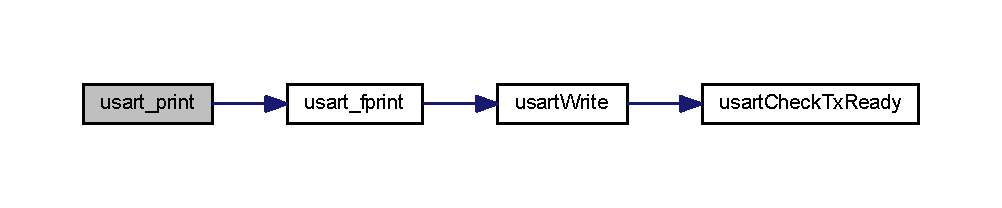
\includegraphics[width=350pt]{group__usart_async_module_ga0f8fdf3d9f7e325fe2297730661facfa_cgraph}
\end{center}
\end{figure}


\index{U\+S\+A\+R\+T Asynchronous Serial Module@{U\+S\+A\+R\+T Asynchronous Serial Module}!usart\+\_\+print\+\_\+\+P@{usart\+\_\+print\+\_\+\+P}}
\index{usart\+\_\+print\+\_\+\+P@{usart\+\_\+print\+\_\+\+P}!U\+S\+A\+R\+T Asynchronous Serial Module@{U\+S\+A\+R\+T Asynchronous Serial Module}}
\subsubsection[{usart\+\_\+print\+\_\+\+P}]{\setlength{\rightskip}{0pt plus 5cm}void usart\+\_\+print\+\_\+\+P (
\begin{DoxyParamCaption}
\item[{P\+G\+M\+\_\+\+P}]{str}
\end{DoxyParamCaption}
)}\label{group__usart_async_module_gae30cd27e2ce82fdb87f06b7460a21b4a}


Print string stored in program memory on default U\+S\+A\+R\+T. 

The function transmits the given string stored in program memory to the default U\+S\+A\+R\+T defined by default\+U\+S\+A\+R\+T with a call to \doxyref{usart\+\_\+fprint\+\_\+\+P()}{p.}{group__usart_async_module_gaa376b136593fb6bc0e5e9f7b35473f14}. 
\begin{DoxyParams}{Parameters}
{\em str} & \\
\hline
\end{DoxyParams}


Here is the call graph for this function\+:\nopagebreak
\begin{figure}[H]
\begin{center}
\leavevmode
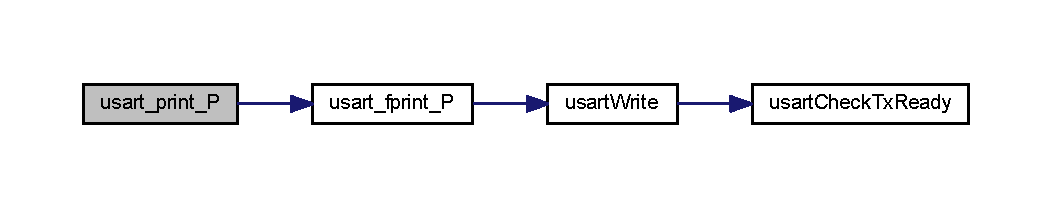
\includegraphics[width=350pt]{group__usart_async_module_gae30cd27e2ce82fdb87f06b7460a21b4a_cgraph}
\end{center}
\end{figure}


\index{U\+S\+A\+R\+T Asynchronous Serial Module@{U\+S\+A\+R\+T Asynchronous Serial Module}!usart\+\_\+printf@{usart\+\_\+printf}}
\index{usart\+\_\+printf@{usart\+\_\+printf}!U\+S\+A\+R\+T Asynchronous Serial Module@{U\+S\+A\+R\+T Asynchronous Serial Module}}
\subsubsection[{usart\+\_\+printf}]{\setlength{\rightskip}{0pt plus 5cm}void usart\+\_\+printf (
\begin{DoxyParamCaption}
\item[{const char $\ast$}]{format, }
\item[{}]{...}
\end{DoxyParamCaption}
)}\label{group__usart_async_module_ga505b60744b81631de13750ca9f5ea1c4}


Standard printf function. 

This function has a variable list and uses the variable list feature of C (see documentation on stdarg). This function calls usart\+\_\+fprintf using the U\+S\+A\+R\+T identifier provided by default\+U\+S\+A\+R\+T. 
\begin{DoxyParams}{Parameters}
{\em format} & -\/ formatting string \\
\hline
\end{DoxyParams}
\index{U\+S\+A\+R\+T Asynchronous Serial Module@{U\+S\+A\+R\+T Asynchronous Serial Module}!usart\+\_\+printf\+\_\+\+P@{usart\+\_\+printf\+\_\+\+P}}
\index{usart\+\_\+printf\+\_\+\+P@{usart\+\_\+printf\+\_\+\+P}!U\+S\+A\+R\+T Asynchronous Serial Module@{U\+S\+A\+R\+T Asynchronous Serial Module}}
\subsubsection[{usart\+\_\+printf\+\_\+\+P}]{\setlength{\rightskip}{0pt plus 5cm}void usart\+\_\+printf\+\_\+\+P (
\begin{DoxyParamCaption}
\item[{P\+G\+M\+\_\+\+P}]{format, }
\item[{}]{...}
\end{DoxyParamCaption}
)}\label{group__usart_async_module_ga0441186875e726f93752dd8e0e95f443}


Standard printf function that uses a formating string stored in memory. 

The function calls usart\+\_\+fprintf\+\_\+\+P to print to the U\+S\+A\+R\+T defined with default\+U\+S\+A\+R\+T. 
\begin{DoxyParams}{Parameters}
{\em format} & \\
\hline
\end{DoxyParams}
\index{U\+S\+A\+R\+T Asynchronous Serial Module@{U\+S\+A\+R\+T Asynchronous Serial Module}!usart\+\_\+rx\+\_\+isr@{usart\+\_\+rx\+\_\+isr}}
\index{usart\+\_\+rx\+\_\+isr@{usart\+\_\+rx\+\_\+isr}!U\+S\+A\+R\+T Asynchronous Serial Module@{U\+S\+A\+R\+T Asynchronous Serial Module}}
\subsubsection[{usart\+\_\+rx\+\_\+isr}]{\setlength{\rightskip}{0pt plus 5cm}void usart\+\_\+rx\+\_\+isr (
\begin{DoxyParamCaption}
\item[{U\+S\+A\+R\+T\+\_\+\+I\+D}]{usart\+Id}
\end{DoxyParamCaption}
)}\label{group__usart_async_module_ga6e2b4d1b6f5bd3b8cf8a9ad223ad348f}
Interrupt service routine for character reception. Saves a received character in the receive ring buffer. If an error occurred, nothing is done. If the ring buffer is full, the character is lost. 
\begin{DoxyParams}{Parameters}
{\em usart\+Id} & -\/ U\+S\+A\+R\+T id \\
\hline
\end{DoxyParams}
\index{U\+S\+A\+R\+T Asynchronous Serial Module@{U\+S\+A\+R\+T Asynchronous Serial Module}!usart\+\_\+tx\+\_\+isr@{usart\+\_\+tx\+\_\+isr}}
\index{usart\+\_\+tx\+\_\+isr@{usart\+\_\+tx\+\_\+isr}!U\+S\+A\+R\+T Asynchronous Serial Module@{U\+S\+A\+R\+T Asynchronous Serial Module}}
\subsubsection[{usart\+\_\+tx\+\_\+isr}]{\setlength{\rightskip}{0pt plus 5cm}void usart\+\_\+tx\+\_\+isr (
\begin{DoxyParamCaption}
\item[{U\+S\+A\+R\+T\+\_\+\+I\+D}]{usart\+Id}
\end{DoxyParamCaption}
)}\label{group__usart_async_module_gacc2987796aa72246682121ad6686c67b}
Interrupt service routine for character transmission. Transmits a character from the transmit ring buffer. If the buffer is empty, the transmit interrupt is disabled. 
\begin{DoxyParams}{Parameters}
{\em usart\+Id} & -\/ U\+S\+A\+R\+T id \\
\hline
\end{DoxyParams}


Here is the call graph for this function\+:\nopagebreak
\begin{figure}[H]
\begin{center}
\leavevmode
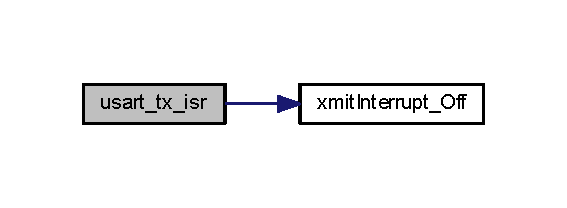
\includegraphics[width=272pt]{group__usart_async_module_gacc2987796aa72246682121ad6686c67b_cgraph}
\end{center}
\end{figure}


\index{U\+S\+A\+R\+T Asynchronous Serial Module@{U\+S\+A\+R\+T Asynchronous Serial Module}!usart\+\_\+xflush\+Rx@{usart\+\_\+xflush\+Rx}}
\index{usart\+\_\+xflush\+Rx@{usart\+\_\+xflush\+Rx}!U\+S\+A\+R\+T Asynchronous Serial Module@{U\+S\+A\+R\+T Asynchronous Serial Module}}
\subsubsection[{usart\+\_\+xflush\+Rx}]{\setlength{\rightskip}{0pt plus 5cm}void usart\+\_\+xflush\+Rx (
\begin{DoxyParamCaption}
\item[{U\+S\+A\+R\+T\+\_\+\+I\+D}]{usart\+Id}
\end{DoxyParamCaption}
)}\label{group__usart_async_module_ga70e50f1bc6f1abd0cb57c53145a0f06e}


Flushes all characters in the receive ring buffer (i.\+e. empties the buffer). 

All characters in the receive ring buffer are discarded. If characters are waiting in the U\+S\+A\+R\+T for reading (a 2 byte F\+I\+F\+O is used for buffering received characters, they are also discarded.


\begin{DoxyParams}{Parameters}
{\em usart\+Id} & -\/ U\+S\+A\+R\+T identifier. \\
\hline
\end{DoxyParams}
\index{U\+S\+A\+R\+T Asynchronous Serial Module@{U\+S\+A\+R\+T Asynchronous Serial Module}!usart\+\_\+xfprint@{usart\+\_\+xfprint}}
\index{usart\+\_\+xfprint@{usart\+\_\+xfprint}!U\+S\+A\+R\+T Asynchronous Serial Module@{U\+S\+A\+R\+T Asynchronous Serial Module}}
\subsubsection[{usart\+\_\+xfprint}]{\setlength{\rightskip}{0pt plus 5cm}void usart\+\_\+xfprint (
\begin{DoxyParamCaption}
\item[{U\+S\+A\+R\+T\+\_\+\+I\+D}]{usart\+Id, }
\item[{uint8\+\_\+t $\ast$}]{str}
\end{DoxyParamCaption}
)}\label{group__usart_async_module_ga7d6d42b48e50bdd87aecab0dc2a9feb6}


Print string to specific U\+S\+A\+R\+T. 

Adds the passed string to the ring buffer using usart\+\_\+xput\+Char. 
\begin{DoxyParams}{Parameters}
{\em usart\+Id} & \\
\hline
{\em str} & \\
\hline
\end{DoxyParams}


Here is the call graph for this function\+:\nopagebreak
\begin{figure}[H]
\begin{center}
\leavevmode
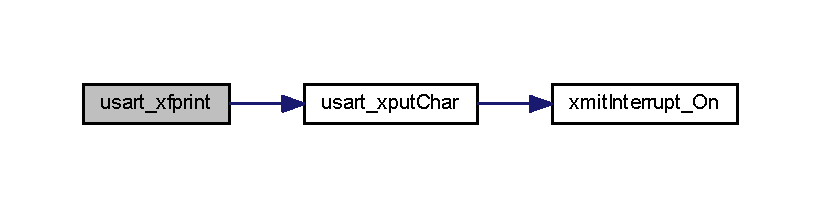
\includegraphics[width=350pt]{group__usart_async_module_ga7d6d42b48e50bdd87aecab0dc2a9feb6_cgraph}
\end{center}
\end{figure}


\index{U\+S\+A\+R\+T Asynchronous Serial Module@{U\+S\+A\+R\+T Asynchronous Serial Module}!usart\+\_\+xfprint\+\_\+\+P@{usart\+\_\+xfprint\+\_\+\+P}}
\index{usart\+\_\+xfprint\+\_\+\+P@{usart\+\_\+xfprint\+\_\+\+P}!U\+S\+A\+R\+T Asynchronous Serial Module@{U\+S\+A\+R\+T Asynchronous Serial Module}}
\subsubsection[{usart\+\_\+xfprint\+\_\+\+P}]{\setlength{\rightskip}{0pt plus 5cm}void usart\+\_\+xfprint\+\_\+\+P (
\begin{DoxyParamCaption}
\item[{U\+S\+A\+R\+T\+\_\+\+I\+D}]{usart\+Id, }
\item[{P\+G\+M\+\_\+\+P}]{str}
\end{DoxyParamCaption}
)}\label{group__usart_async_module_gae8212e8aca5b91172440dc3735dd7ba4}


Print string stored in program memory to specific U\+S\+A\+R\+T. 

Adds the passed string to the ring buffer using usart\+\_\+xput\+Char. 
\begin{DoxyParams}{Parameters}
{\em usart\+Id} & -\/ U\+S\+A\+R\+T identifier. \\
\hline
{\em str} & -\/ Reference to string stored in program memory. \\
\hline
\end{DoxyParams}


Here is the call graph for this function\+:\nopagebreak
\begin{figure}[H]
\begin{center}
\leavevmode
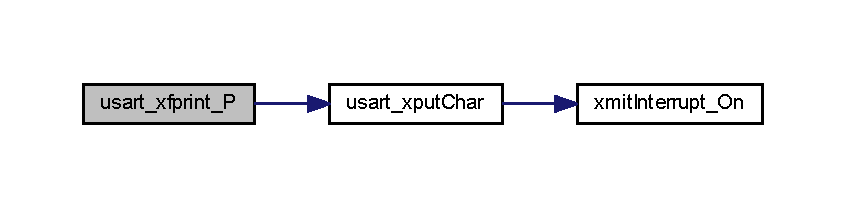
\includegraphics[width=350pt]{group__usart_async_module_gae8212e8aca5b91172440dc3735dd7ba4_cgraph}
\end{center}
\end{figure}


\index{U\+S\+A\+R\+T Asynchronous Serial Module@{U\+S\+A\+R\+T Asynchronous Serial Module}!usart\+\_\+xfprintf@{usart\+\_\+xfprintf}}
\index{usart\+\_\+xfprintf@{usart\+\_\+xfprintf}!U\+S\+A\+R\+T Asynchronous Serial Module@{U\+S\+A\+R\+T Asynchronous Serial Module}}
\subsubsection[{usart\+\_\+xfprintf}]{\setlength{\rightskip}{0pt plus 5cm}void usart\+\_\+xfprintf (
\begin{DoxyParamCaption}
\item[{int}]{usart\+Id, }
\item[{const char $\ast$}]{format, }
\item[{}]{...}
\end{DoxyParamCaption}
)}\label{group__usart_async_module_ga94601796b62f88f4364afbc1ed037d10}


Standard printf function for specific U\+S\+A\+R\+T. 

This function has a variable list and uses the variable list feature of C (see documentation on stdarg). The function uses vsnprintf function for formating the string to output in the work\+Buffer before transmission. This function calls usart\+\_\+fprint\+\_\+\+P to send the contents of the work buffer to the U\+S\+A\+R\+T.


\begin{DoxyParams}{Parameters}
{\em usart\+Id} & -\/ U\+S\+A\+R\+T Identifier -\/ note that var\+\_\+list, va\+\_\+start, etc does not work when using U\+S\+E\+R\+I\+D enumerated types. must be an int. \\
\hline
{\em format} & -\/ Formating string. \\
\hline
\end{DoxyParams}
\index{U\+S\+A\+R\+T Asynchronous Serial Module@{U\+S\+A\+R\+T Asynchronous Serial Module}!usart\+\_\+xfprintf\+\_\+\+P@{usart\+\_\+xfprintf\+\_\+\+P}}
\index{usart\+\_\+xfprintf\+\_\+\+P@{usart\+\_\+xfprintf\+\_\+\+P}!U\+S\+A\+R\+T Asynchronous Serial Module@{U\+S\+A\+R\+T Asynchronous Serial Module}}
\subsubsection[{usart\+\_\+xfprintf\+\_\+\+P}]{\setlength{\rightskip}{0pt plus 5cm}void usart\+\_\+xfprintf\+\_\+\+P (
\begin{DoxyParamCaption}
\item[{int}]{usart\+Id, }
\item[{P\+G\+M\+\_\+\+P}]{format, }
\item[{}]{...}
\end{DoxyParamCaption}
)}\label{group__usart_async_module_ga8092a20ae9bed598702da288b55c80c6}


Standard printf function for specific U\+S\+A\+R\+T that uses a formating string stored in program memory. 

This function has a variable list and uses the variable list feature of C (see documentation on stdarg). The function uses vsnprintf\+\_\+\+P function for formating the string to output in the work\+Buffer before transmission. This function calls usart\+\_\+fprint\+\_\+\+P to send the contents of the work buffer to the U\+S\+A\+R\+T. The formating string is stored in program memory. 
\begin{DoxyParams}{Parameters}
{\em usart\+Id} & -\/ U\+S\+A\+R\+T identifier -\/ note that var\+\_\+list, va\+\_\+start, etc does not work when using U\+S\+E\+R\+I\+D enumerated types. must be an int. \\
\hline
{\em format} & -\/ Formating String. \\
\hline
\end{DoxyParams}
\index{U\+S\+A\+R\+T Asynchronous Serial Module@{U\+S\+A\+R\+T Asynchronous Serial Module}!usart\+\_\+xget\+Char@{usart\+\_\+xget\+Char}}
\index{usart\+\_\+xget\+Char@{usart\+\_\+xget\+Char}!U\+S\+A\+R\+T Asynchronous Serial Module@{U\+S\+A\+R\+T Asynchronous Serial Module}}
\subsubsection[{usart\+\_\+xget\+Char}]{\setlength{\rightskip}{0pt plus 5cm}U\+Base\+Type\+\_\+t usart\+\_\+xget\+Char (
\begin{DoxyParamCaption}
\item[{U\+S\+A\+R\+T\+\_\+\+I\+D}]{usart\+Id, }
\item[{U\+Base\+Type\+\_\+t $\ast$}]{pc\+Rxed\+Char}
\end{DoxyParamCaption}
)}\label{group__usart_async_module_ga3958a2e258e69977428337f1b79b559d}


Get a character from the reception ring buffer. 

The retrieved character if available is stored using pointer pc\+Rxed\+Char. The function returns pd\+T\+R\+U\+E if a character was available and pd\+F\+A\+L\+S\+E otherwise (in this latter case, the contents referenced by pc\+Rxed\+Char are not changed). 
\begin{DoxyParams}{Parameters}
{\em usart\+Id} & -\/ U\+S\+A\+R\+T identifier \\
\hline
{\em pc\+Rxed\+Char} & -\/ pointer for storing character read. \\
\hline
\end{DoxyParams}
\begin{DoxyReturn}{Returns}
pd\+F\+A\+L\+S\+E if a character was available in the reception ring buffer (stored at pc\+R\+Xed\+Char) and pd\+F\+A\+L\+S\+E otherwise. 
\end{DoxyReturn}
\index{U\+S\+A\+R\+T Asynchronous Serial Module@{U\+S\+A\+R\+T Asynchronous Serial Module}!usart\+\_\+xprint@{usart\+\_\+xprint}}
\index{usart\+\_\+xprint@{usart\+\_\+xprint}!U\+S\+A\+R\+T Asynchronous Serial Module@{U\+S\+A\+R\+T Asynchronous Serial Module}}
\subsubsection[{usart\+\_\+xprint}]{\setlength{\rightskip}{0pt plus 5cm}void usart\+\_\+xprint (
\begin{DoxyParamCaption}
\item[{uint8\+\_\+t $\ast$}]{str}
\end{DoxyParamCaption}
)}\label{group__usart_async_module_gab5e44adf779c82fd1c56fb8bca7bffb7}


Prints a string on the default U\+S\+A\+R\+T (defined by default\+U\+S\+A\+R\+T). 

Uses a call to usart\+\_\+xfprint to print a string referenced by str. The string is stored in the transmission ring buffer for transmission with the I\+S\+Rs. 
\begin{DoxyParams}{Parameters}
{\em str} & -\/ Pointer to string. \\
\hline
\end{DoxyParams}


Here is the call graph for this function\+:\nopagebreak
\begin{figure}[H]
\begin{center}
\leavevmode
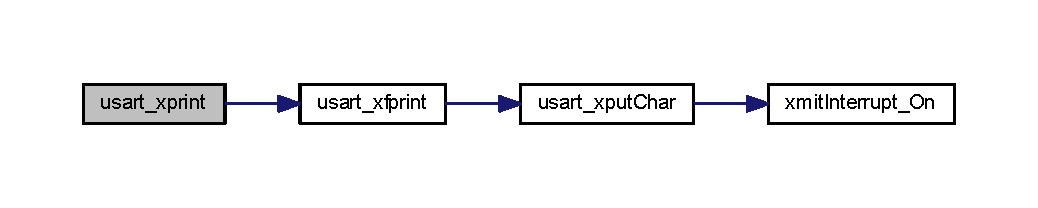
\includegraphics[width=350pt]{group__usart_async_module_gab5e44adf779c82fd1c56fb8bca7bffb7_cgraph}
\end{center}
\end{figure}


\index{U\+S\+A\+R\+T Asynchronous Serial Module@{U\+S\+A\+R\+T Asynchronous Serial Module}!usart\+\_\+xprint\+\_\+\+P@{usart\+\_\+xprint\+\_\+\+P}}
\index{usart\+\_\+xprint\+\_\+\+P@{usart\+\_\+xprint\+\_\+\+P}!U\+S\+A\+R\+T Asynchronous Serial Module@{U\+S\+A\+R\+T Asynchronous Serial Module}}
\subsubsection[{usart\+\_\+xprint\+\_\+\+P}]{\setlength{\rightskip}{0pt plus 5cm}void usart\+\_\+xprint\+\_\+\+P (
\begin{DoxyParamCaption}
\item[{P\+G\+M\+\_\+\+P}]{str}
\end{DoxyParamCaption}
)}\label{group__usart_async_module_ga27ada721bb00993418f8e3ffb1152d52}


Prints a string stored in program memory on the default U\+S\+A\+R\+T (defined by default\+U\+S\+A\+R\+T). 

Uses a call to usart\+\_\+xfprint\+\_\+\+P to print a string referenced by str. The string is stored in the transmission ring buffer for transmission with the I\+S\+Rs. 
\begin{DoxyParams}{Parameters}
{\em str} & -\/ Pointer to string in program memory. \\
\hline
\end{DoxyParams}


Here is the call graph for this function\+:\nopagebreak
\begin{figure}[H]
\begin{center}
\leavevmode
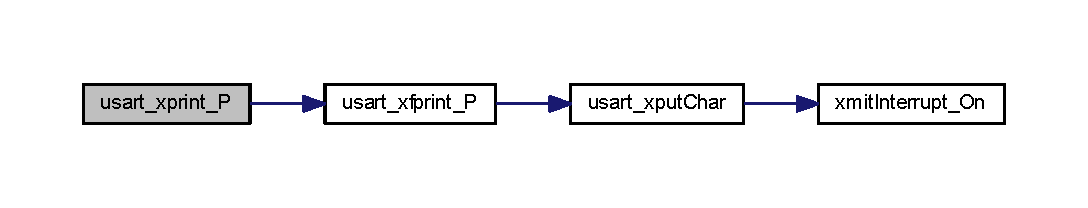
\includegraphics[width=350pt]{group__usart_async_module_ga27ada721bb00993418f8e3ffb1152d52_cgraph}
\end{center}
\end{figure}


\index{U\+S\+A\+R\+T Asynchronous Serial Module@{U\+S\+A\+R\+T Asynchronous Serial Module}!usart\+\_\+xprintf@{usart\+\_\+xprintf}}
\index{usart\+\_\+xprintf@{usart\+\_\+xprintf}!U\+S\+A\+R\+T Asynchronous Serial Module@{U\+S\+A\+R\+T Asynchronous Serial Module}}
\subsubsection[{usart\+\_\+xprintf}]{\setlength{\rightskip}{0pt plus 5cm}void usart\+\_\+xprintf (
\begin{DoxyParamCaption}
\item[{const char $\ast$}]{format, }
\item[{}]{...}
\end{DoxyParamCaption}
)}\label{group__usart_async_module_ga9ec472642da5fe42928fb1d81e3115cd}


Standard printf (interrupt driven) to default U\+S\+A\+R\+T. 

Formats and prints string on default U\+S\+A\+R\+T (default\+U\+S\+A\+R\+T) using the usart\+\_\+xfprintf function. 
\begin{DoxyParams}{Parameters}
{\em format} & -\/ Formatting string. The string is stored in the transmission ring buffer for transmission with the I\+S\+Rs. \\
\hline
\end{DoxyParams}
\index{U\+S\+A\+R\+T Asynchronous Serial Module@{U\+S\+A\+R\+T Asynchronous Serial Module}!usart\+\_\+xprintf\+\_\+\+P@{usart\+\_\+xprintf\+\_\+\+P}}
\index{usart\+\_\+xprintf\+\_\+\+P@{usart\+\_\+xprintf\+\_\+\+P}!U\+S\+A\+R\+T Asynchronous Serial Module@{U\+S\+A\+R\+T Asynchronous Serial Module}}
\subsubsection[{usart\+\_\+xprintf\+\_\+\+P}]{\setlength{\rightskip}{0pt plus 5cm}void usart\+\_\+xprintf\+\_\+\+P (
\begin{DoxyParamCaption}
\item[{P\+G\+M\+\_\+\+P}]{format, }
\item[{}]{...}
\end{DoxyParamCaption}
)}\label{group__usart_async_module_gaf7d0d5b028d30f55439119f42ad7ed69}


Standard printf (interrupt driven) to default U\+S\+A\+R\+T using formating string stored in program memory. 

Formats and prints string on default U\+S\+A\+R\+T (default\+U\+S\+A\+R\+T) using the usart\+\_\+xfprintf\+\_\+\+P function. 
\begin{DoxyParams}{Parameters}
{\em format} & -\/ Formatting string stored in program memory. The string is stored in the transmission ring buffer for transmission with the I\+S\+Rs. \\
\hline
\end{DoxyParams}
\index{U\+S\+A\+R\+T Asynchronous Serial Module@{U\+S\+A\+R\+T Asynchronous Serial Module}!usart\+\_\+xput\+Char@{usart\+\_\+xput\+Char}}
\index{usart\+\_\+xput\+Char@{usart\+\_\+xput\+Char}!U\+S\+A\+R\+T Asynchronous Serial Module@{U\+S\+A\+R\+T Asynchronous Serial Module}}
\subsubsection[{usart\+\_\+xput\+Char}]{\setlength{\rightskip}{0pt plus 5cm}U\+Base\+Type\+\_\+t usart\+\_\+xput\+Char (
\begin{DoxyParamCaption}
\item[{U\+S\+A\+R\+T\+\_\+\+I\+D}]{usart\+Id, }
\item[{const U\+Base\+Type\+\_\+t}]{c\+Out\+Char}
\end{DoxyParamCaption}
)}\label{group__usart_async_module_ga520a2c4212a37daf9f42e747a7ff420f}


Drops a character into the transmit ring buffer. 

If the ring buffer is full, the function delays to allow transmission of characters to free up space in buffer. The function turns on the transmit interrupt for the U\+S\+A\+R\+T. 
\begin{DoxyParams}{Parameters}
{\em usart\+Id} & \\
\hline
{\em c\+Out\+Char} & \\
\hline
\end{DoxyParams}
\begin{DoxyReturn}{Returns}

\end{DoxyReturn}


Here is the call graph for this function\+:\nopagebreak
\begin{figure}[H]
\begin{center}
\leavevmode
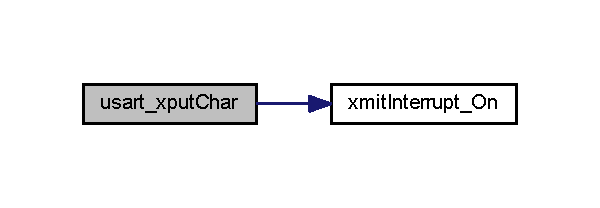
\includegraphics[width=288pt]{group__usart_async_module_ga520a2c4212a37daf9f42e747a7ff420f_cgraph}
\end{center}
\end{figure}


\index{U\+S\+A\+R\+T Asynchronous Serial Module@{U\+S\+A\+R\+T Asynchronous Serial Module}!usart\+Check\+Rx\+Complete@{usart\+Check\+Rx\+Complete}}
\index{usart\+Check\+Rx\+Complete@{usart\+Check\+Rx\+Complete}!U\+S\+A\+R\+T Asynchronous Serial Module@{U\+S\+A\+R\+T Asynchronous Serial Module}}
\subsubsection[{usart\+Check\+Rx\+Complete}]{\setlength{\rightskip}{0pt plus 5cm}int8\+\_\+t usart\+Check\+Rx\+Complete (
\begin{DoxyParamCaption}
\item[{U\+S\+A\+R\+T\+\_\+\+I\+D}]{usart\+Id}
\end{DoxyParamCaption}
)\hspace{0.3cm}{\ttfamily [inline]}}\label{group__usart_async_module_ga590146f26805ddb1810fe874188aa10d}


Check if reception is complete. The function returns the status of the R\+X\+C bit of the U\+S\+A\+R\+T. When set, the bit indicates that data can be read from the U\+S\+A\+R\+T. 


\begin{DoxyParams}{Parameters}
{\em usart\+Id} & -\/ identifier of the usart (see U\+S\+A\+R\+T\+\_\+\+I\+D type; used with usart\+Reg array to get pointer to control register U\+C\+S\+R\+A. \\
\hline
\end{DoxyParams}
\begin{DoxyReturn}{Returns}
-\/ status of the R\+S\+C bit, if non-\/zero, the U\+S\+A\+R\+T has received data and the data register can be read. 
\end{DoxyReturn}
\index{U\+S\+A\+R\+T Asynchronous Serial Module@{U\+S\+A\+R\+T Asynchronous Serial Module}!usart\+Check\+Tx\+Ready@{usart\+Check\+Tx\+Ready}}
\index{usart\+Check\+Tx\+Ready@{usart\+Check\+Tx\+Ready}!U\+S\+A\+R\+T Asynchronous Serial Module@{U\+S\+A\+R\+T Asynchronous Serial Module}}
\subsubsection[{usart\+Check\+Tx\+Ready}]{\setlength{\rightskip}{0pt plus 5cm}int8\+\_\+t usart\+Check\+Tx\+Ready (
\begin{DoxyParamCaption}
\item[{U\+S\+A\+R\+T\+\_\+\+I\+D}]{usart\+Id}
\end{DoxyParamCaption}
)\hspace{0.3cm}{\ttfamily [inline]}}\label{group__usart_async_module_gaaab3f24aac455dad2295e72f6dff7bb5}


Check if transmission is complete. The function returns the status of the U\+D\+R\+E bit of the U\+S\+A\+R\+T. When set, the bit indicates that data can be written to the U\+S\+A\+R\+T. 


\begin{DoxyParams}{Parameters}
{\em usart\+Id} & -\/ identifier of the usart (see U\+S\+A\+R\+T\+\_\+\+I\+D type; used with usart\+Reg array to get pointer to control register U\+C\+S\+R\+A. \\
\hline
\end{DoxyParams}
\begin{DoxyReturn}{Returns}
-\/ status of the U\+D\+R\+E bit, if non-\/zero, the U\+S\+A\+R\+T, data for transmission can be written to the transmit register U\+D\+R\+E. 
\end{DoxyReturn}
\index{U\+S\+A\+R\+T Asynchronous Serial Module@{U\+S\+A\+R\+T Asynchronous Serial Module}!usart\+Close@{usart\+Close}}
\index{usart\+Close@{usart\+Close}!U\+S\+A\+R\+T Asynchronous Serial Module@{U\+S\+A\+R\+T Asynchronous Serial Module}}
\subsubsection[{usart\+Close}]{\setlength{\rightskip}{0pt plus 5cm}void usart\+Close (
\begin{DoxyParamCaption}
\item[{U\+S\+A\+R\+T\+\_\+\+I\+D}]{usart\+Id}
\end{DoxyParamCaption}
)}\label{group__usart_async_module_ga6343cf3035ec8972e44716a951a29d42}


Close a connection on a U\+S\+A\+R\+T. 

The buffers allocated to the connection are released. U\+S\+A\+R\+T registers are configure to turn off reception and transmission. Interrups are also turned off. 
\begin{DoxyParams}{Parameters}
{\em usart\+Id} & \\
\hline
\end{DoxyParams}


Here is the call graph for this function\+:\nopagebreak
\begin{figure}[H]
\begin{center}
\leavevmode
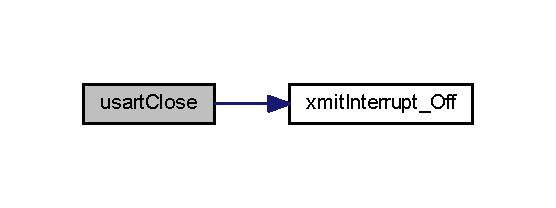
\includegraphics[width=267pt]{group__usart_async_module_ga6343cf3035ec8972e44716a951a29d42_cgraph}
\end{center}
\end{figure}


\index{U\+S\+A\+R\+T Asynchronous Serial Module@{U\+S\+A\+R\+T Asynchronous Serial Module}!usart\+Open@{usart\+Open}}
\index{usart\+Open@{usart\+Open}!U\+S\+A\+R\+T Asynchronous Serial Module@{U\+S\+A\+R\+T Asynchronous Serial Module}}
\subsubsection[{usart\+Open}]{\setlength{\rightskip}{0pt plus 5cm}U\+S\+A\+R\+T\+\_\+\+I\+D usart\+Open (
\begin{DoxyParamCaption}
\item[{U\+S\+A\+R\+T\+\_\+\+I\+D}]{usart\+Id, }
\item[{uint32\+\_\+t}]{ul\+Wanted\+Baud, }
\item[{uint16\+\_\+t}]{ux\+Tx\+Queue\+Length, }
\item[{uint16\+\_\+t}]{ux\+Rx\+Queue\+Length}
\end{DoxyParamCaption}
)}\label{group__usart_async_module_gae9acc73d962adef7e91a498618ff012f}


Open a connection on a U\+S\+A\+R\+T. 

Sets up the connection for both transmission and reception. All buffers for supporting communications are allocated and control registers of the U\+S\+A\+R\+T\+S initialised for both transmission and reception.


\begin{DoxyParams}{Parameters}
{\em usart\+Id} & -\/ U\+S\+A\+R\+T identifier. \\
\hline
{\em ul\+Wanted\+Baud} & -\/ U\+S\+A\+R\+T bit rate (units of bits/second) \\
\hline
{\em ux\+Tx\+Queue\+Length} & -\/ length of the transmission ring buffer (also sets the length of the work buffer) \\
\hline
{\em ux\+Rx\+Queue\+Length} & -\/ length of the reception ring buffer \\
\hline
\end{DoxyParams}
\begin{DoxyReturn}{Returns}
Usart identifier. 
\end{DoxyReturn}
\index{U\+S\+A\+R\+T Asynchronous Serial Module@{U\+S\+A\+R\+T Asynchronous Serial Module}!usart\+Read@{usart\+Read}}
\index{usart\+Read@{usart\+Read}!U\+S\+A\+R\+T Asynchronous Serial Module@{U\+S\+A\+R\+T Asynchronous Serial Module}}
\subsubsection[{usart\+Read}]{\setlength{\rightskip}{0pt plus 5cm}int8\+\_\+t usart\+Read (
\begin{DoxyParamCaption}
\item[{U\+S\+A\+R\+T\+\_\+\+I\+D}]{usart\+Id}
\end{DoxyParamCaption}
)}\label{group__usart_async_module_ga152b8198df4c2d75e34547a8c13c7457}


Low level read function (single character). Delays until data available from the U\+S\+A\+R\+T. Will check for reception errors. 


\begin{DoxyParams}{Parameters}
{\em usart\+Id} & -\/ identifier of the usart (see U\+S\+A\+R\+T\+\_\+\+I\+D type; used with usart\+Reg array to get pointer to data register U\+D\+R. \\
\hline
\end{DoxyParams}
\begin{DoxyReturn}{Returns}
8-\/bit data received and read from the U\+D\+R register. Returns -\/ 0x\+F\+F if an error occured. 
\end{DoxyReturn}


Here is the call graph for this function\+:\nopagebreak
\begin{figure}[H]
\begin{center}
\leavevmode
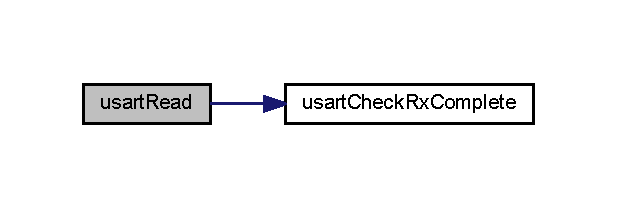
\includegraphics[width=296pt]{group__usart_async_module_ga152b8198df4c2d75e34547a8c13c7457_cgraph}
\end{center}
\end{figure}


\index{U\+S\+A\+R\+T Asynchronous Serial Module@{U\+S\+A\+R\+T Asynchronous Serial Module}!usart\+Write@{usart\+Write}}
\index{usart\+Write@{usart\+Write}!U\+S\+A\+R\+T Asynchronous Serial Module@{U\+S\+A\+R\+T Asynchronous Serial Module}}
\subsubsection[{usart\+Write}]{\setlength{\rightskip}{0pt plus 5cm}void usart\+Write (
\begin{DoxyParamCaption}
\item[{U\+S\+A\+R\+T\+\_\+\+I\+D}]{usart\+Id, }
\item[{int8\+\_\+t}]{data\+Out}
\end{DoxyParamCaption}
)}\label{group__usart_async_module_ga12dffa6d7df2b7e6049e3bc08b939e07}


Low level write function (single character). Will delay until usart is ready to accept the 8 bit data. 


\begin{DoxyParams}{Parameters}
{\em usart\+Id} & -\/ identifier of the usart (see U\+S\+A\+R\+T\+\_\+\+I\+D type; used with usart\+Reg array to get pointer to data register U\+D\+R. \\
\hline
{\em data\+Out} & -\/ the 8-\/bit data to write to the data register. \\
\hline
\end{DoxyParams}


Here is the call graph for this function\+:\nopagebreak
\begin{figure}[H]
\begin{center}
\leavevmode
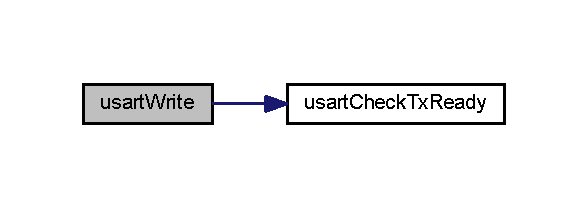
\includegraphics[width=282pt]{group__usart_async_module_ga12dffa6d7df2b7e6049e3bc08b939e07_cgraph}
\end{center}
\end{figure}


\index{U\+S\+A\+R\+T Asynchronous Serial Module@{U\+S\+A\+R\+T Asynchronous Serial Module}!xmit\+Interrupt\+\_\+\+Off@{xmit\+Interrupt\+\_\+\+Off}}
\index{xmit\+Interrupt\+\_\+\+Off@{xmit\+Interrupt\+\_\+\+Off}!U\+S\+A\+R\+T Asynchronous Serial Module@{U\+S\+A\+R\+T Asynchronous Serial Module}}
\subsubsection[{xmit\+Interrupt\+\_\+\+Off}]{\setlength{\rightskip}{0pt plus 5cm}void xmit\+Interrupt\+\_\+\+Off (
\begin{DoxyParamCaption}
\item[{U\+S\+A\+R\+T\+\_\+\+I\+D}]{usart\+Id}
\end{DoxyParamCaption}
)\hspace{0.3cm}{\ttfamily [inline]}}\label{group__usart_async_module_ga47ace99c93e8f4b284443b758cab1523}
Turns off the transmit interrupt for a U\+S\+A\+R\+T. Clears the U\+D\+R\+I\+E bit in the control and status register U\+C\+S\+R\+B which disables the interrupt when the transmit data register is empty. 
\begin{DoxyParams}{Parameters}
{\em usart\+Id} & -\/ U\+S\+A\+R\+T identifier \\
\hline
\end{DoxyParams}
\index{U\+S\+A\+R\+T Asynchronous Serial Module@{U\+S\+A\+R\+T Asynchronous Serial Module}!xmit\+Interrupt\+\_\+\+On@{xmit\+Interrupt\+\_\+\+On}}
\index{xmit\+Interrupt\+\_\+\+On@{xmit\+Interrupt\+\_\+\+On}!U\+S\+A\+R\+T Asynchronous Serial Module@{U\+S\+A\+R\+T Asynchronous Serial Module}}
\subsubsection[{xmit\+Interrupt\+\_\+\+On}]{\setlength{\rightskip}{0pt plus 5cm}void xmit\+Interrupt\+\_\+\+On (
\begin{DoxyParamCaption}
\item[{U\+S\+A\+R\+T\+\_\+\+I\+D}]{usart\+Id}
\end{DoxyParamCaption}
)\hspace{0.3cm}{\ttfamily [inline]}}\label{group__usart_async_module_gaddeaba370b80a1dd990f7f713ba7303f}
Turns on the transmit interrupt for a U\+S\+A\+R\+T Sets the U\+D\+R\+I\+E bit in the control and status register U\+C\+S\+R\+B which configures the U\+S\+A\+R\+T to generate an interrupt when the transmit data register is empty, i.\+e. can write a character to the transmit register (U\+D\+R) for transmission. The receive interrupt is enabled when the U\+S\+A\+R\+T is configured. 
\begin{DoxyParams}{Parameters}
{\em usart\+Id} & -\/ U\+S\+A\+R\+T identifier \\
\hline
\end{DoxyParams}


\subsection{Variable Documentation}
\index{U\+S\+A\+R\+T Asynchronous Serial Module@{U\+S\+A\+R\+T Asynchronous Serial Module}!default\+U\+S\+A\+R\+T@{default\+U\+S\+A\+R\+T}}
\index{default\+U\+S\+A\+R\+T@{default\+U\+S\+A\+R\+T}!U\+S\+A\+R\+T Asynchronous Serial Module@{U\+S\+A\+R\+T Asynchronous Serial Module}}
\subsubsection[{default\+U\+S\+A\+R\+T}]{\setlength{\rightskip}{0pt plus 5cm}U\+S\+A\+R\+T\+\_\+\+I\+D default\+U\+S\+A\+R\+T = U\+S\+A\+R\+T0}\label{group__usart_async_module_ga88cfc7c9ded2bea56fff795fe46b68c0}
Default U\+S\+A\+R\+T Can be changed using \doxyref{set\+Default\+U\+S\+A\+R\+T()}{p.}{group__usart_async_module_gaa679900a334c7873eb71c86fe52cbf40} \index{U\+S\+A\+R\+T Asynchronous Serial Module@{U\+S\+A\+R\+T Asynchronous Serial Module}!usart\+Com\+Buf@{usart\+Com\+Buf}}
\index{usart\+Com\+Buf@{usart\+Com\+Buf}!U\+S\+A\+R\+T Asynchronous Serial Module@{U\+S\+A\+R\+T Asynchronous Serial Module}}
\subsubsection[{usart\+Com\+Buf}]{\setlength{\rightskip}{0pt plus 5cm}{\bf U\+S\+A\+R\+T\+\_\+\+C\+O\+M\+\_\+\+B\+U\+F} usart\+Com\+Buf[N\+U\+M\+\_\+\+U\+S\+A\+R\+T\+S]}\label{group__usart_async_module_ga01280f1bdc978bbad7a0ae0fca24f0f4}
Array of \doxyref{U\+S\+A\+R\+T\+\_\+\+C\+O\+M\+\_\+\+B\+U\+F}{p.}{struct_u_s_a_r_t___c_o_m___b_u_f} structures that provide buffers for each of the U\+S\+A\+R\+T\textquotesingle{}s. Note that the buffers are allocated an initialised by the usart\+Open function and released by the usart\+Close function. Use the enum U\+S\+A\+R\+T\+\_\+\+I\+D identifiers as indices into the array. \index{U\+S\+A\+R\+T Asynchronous Serial Module@{U\+S\+A\+R\+T Asynchronous Serial Module}!usart\+Reg@{usart\+Reg}}
\index{usart\+Reg@{usart\+Reg}!U\+S\+A\+R\+T Asynchronous Serial Module@{U\+S\+A\+R\+T Asynchronous Serial Module}}
\subsubsection[{usart\+Reg}]{\setlength{\rightskip}{0pt plus 5cm}{\bf U\+S\+A\+R\+T\+\_\+\+R\+E\+G\+I\+S\+T\+E\+R\+S} usart\+Reg[$\,$]}\label{group__usart_async_module_gaf964270351d58d348a34bfec204765cb}
{\bfseries Initial value\+:}
\begin{DoxyCode}
=
\{
        \{ &UDR0, &UCSR0A, &UCSR0B, &UCSR0C, &UBRR0  \},
        \{ &UDR1, &UCSR1A, &UCSR1B, &UCSR1C, &UBRR1  \},
        \{ &UDR2, &UCSR2A, &UCSR2B, &UCSR2C, &UBRR2  \},
        \{ &UDR3, &UCSR3A, &UCSR3B, &UCSR3C, &UBRR3  \}
\}
\end{DoxyCode}
Array of \doxyref{U\+S\+A\+R\+T\+\_\+\+R\+E\+G\+I\+S\+T\+E\+R\+S}{p.}{struct_u_s_a_r_t___r_e_g_i_s_t_e_r_s} structures that defines the references to the registers of all four U\+S\+A\+R\+T\+S. Use the enum U\+S\+A\+R\+T\+\_\+\+I\+D identifiers as indices into the array. 
\chapter{Data Structure Documentation}
\section{encoder\+\_\+config\+\_\+t Struct Reference}
\label{structencoder__config__t}\index{encoder\+\_\+config\+\_\+t@{encoder\+\_\+config\+\_\+t}}


Collaboration diagram for encoder\+\_\+config\+\_\+t\+:\nopagebreak
\begin{figure}[H]
\begin{center}
\leavevmode
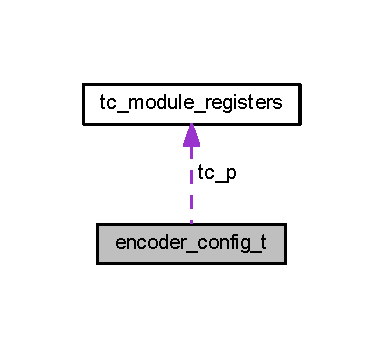
\includegraphics[width=184pt]{structencoder__config__t__coll__graph}
\end{center}
\end{figure}
\subsection*{Data Fields}
\begin{DoxyCompactItemize}
\item 
volatile uint8\+\_\+t $\ast$ {\bfseries P\+O\+R\+T\+\_\+ptr}\label{structencoder__config__t_a9cb2f16ba9ae962a2f4f401f4e53ae72}

\item 
volatile uint8\+\_\+t $\ast$ {\bfseries D\+D\+R\+\_\+ptr}\label{structencoder__config__t_a5dc1a4776f66ab5e5eacce4ccbb048b2}

\item 
uint8\+\_\+t {\bfseries pin}\label{structencoder__config__t_ad48157b503f3847e3b08bc3e204a0d47}

\item 
const struct {\bf tc\+\_\+module\+\_\+registers} $\ast$ {\bfseries tc\+\_\+p}\label{structencoder__config__t_a63ef61b522de661084aca5407037622d}

\end{DoxyCompactItemize}


The documentation for this struct was generated from the following file\+:\begin{DoxyCompactItemize}
\item 
motion.\+c\end{DoxyCompactItemize}

\section{motor\+\_\+registers\+\_\+s Struct Reference}
\label{structmotor__registers__s}\index{motor\+\_\+registers\+\_\+s@{motor\+\_\+registers\+\_\+s}}


Collaboration diagram for motor\+\_\+registers\+\_\+s\+:\nopagebreak
\begin{figure}[H]
\begin{center}
\leavevmode
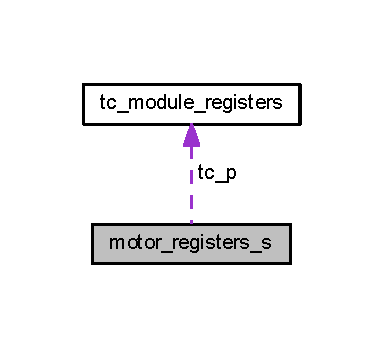
\includegraphics[width=184pt]{structmotor__registers__s__coll__graph}
\end{center}
\end{figure}
\subsection*{Data Fields}
\begin{DoxyCompactItemize}
\item 
volatile uint16\+\_\+t $\ast$ {\bfseries O\+C\+R\+\_\+ptr}\label{structmotor__registers__s_a9e151bedf793f3664a8acb277988f23a}

\item 
volatile uint8\+\_\+t $\ast$ {\bfseries D\+D\+R\+\_\+ptr}\label{structmotor__registers__s_a69a589af1b6e1a8db9758d0f5fa65e37}

\item 
volatile uint8\+\_\+t $\ast$ {\bfseries P\+O\+R\+T\+\_\+ptr}\label{structmotor__registers__s_a530b045599b736fed1e8b6adcb9dcd5f}

\item 
uint8\+\_\+t {\bfseries pin}\label{structmotor__registers__s_a0b1799ba98f3c56dc72f51d490d2b00d}

\item 
uint8\+\_\+t {\bfseries channel}\label{structmotor__registers__s_a759cd205c48cbbd49b0722c44d7a6717}

\item 
const struct {\bf tc\+\_\+module\+\_\+registers} $\ast$ {\bfseries tc\+\_\+p}\label{structmotor__registers__s_a99085fa10e4e9ef7cf0a2537abbd6ab2}

\end{DoxyCompactItemize}


The documentation for this struct was generated from the following file\+:\begin{DoxyCompactItemize}
\item 
motion.\+c\end{DoxyCompactItemize}

\section{tc\+\_\+module\+\_\+registers Struct Reference}
\label{structtc__module__registers}\index{tc\+\_\+module\+\_\+registers@{tc\+\_\+module\+\_\+registers}}
\subsection*{Data Fields}
\begin{DoxyCompactItemize}
\item 
volatile uint8\+\_\+t $\ast$ {\bfseries T\+I\+F\+R\+\_\+ptr}\label{structtc__module__registers_aeedf1046b5839d409a062d57db659be3}

\item 
volatile uint8\+\_\+t $\ast$ {\bfseries T\+I\+M\+S\+K\+\_\+ptr}\label{structtc__module__registers_ae234affdd388677523c04915ce08a7ff}

\item 
volatile uint16\+\_\+t $\ast$ {\bfseries T\+C\+N\+T\+\_\+ptr}\label{structtc__module__registers_afe77818f75c685966eb2164d8e163cce}

\item 
volatile uint16\+\_\+t $\ast$ {\bfseries I\+C\+R\+\_\+ptr}\label{structtc__module__registers_a12038ce56365e723fe183a5331cc3f03}

\item 
volatile uint8\+\_\+t $\ast$ {\bfseries T\+C\+C\+R\+\_\+\+A\+\_\+ptr}\label{structtc__module__registers_a898e9463cefe8762d109f1ef250c5e13}

\item 
volatile uint8\+\_\+t $\ast$ {\bfseries T\+C\+C\+R\+\_\+\+B\+\_\+ptr}\label{structtc__module__registers_a00ac921da136f9af2f1832a4dd243d88}

\item 
uint8\+\_\+t {\bfseries prescale}\label{structtc__module__registers_ab2b985595889f8fc543d56f32d9e8040}

\item 
uint8\+\_\+t {\bfseries wgm\+\_\+mode}\label{structtc__module__registers_a272a3b5aca6bb0aa2190d4f60d979783}

\item 
volatile uint16\+\_\+t $\ast$ {\bfseries T\+O\+P\+\_\+value\+\_\+p}\label{structtc__module__registers_ac0a10e603c390e7ca6ff3935ad364a00}

\end{DoxyCompactItemize}


The documentation for this struct was generated from the following file\+:\begin{DoxyCompactItemize}
\item 
motion.\+c\end{DoxyCompactItemize}

\section{U\+S\+A\+R\+T\+\_\+\+C\+O\+M\+\_\+\+B\+U\+F Struct Reference}
\label{struct_u_s_a_r_t___c_o_m___b_u_f}\index{U\+S\+A\+R\+T\+\_\+\+C\+O\+M\+\_\+\+B\+U\+F@{U\+S\+A\+R\+T\+\_\+\+C\+O\+M\+\_\+\+B\+U\+F}}


Structure of buffers to support communications with a U\+S\+A\+R\+T.  


\subsection*{Data Fields}
\begin{DoxyCompactItemize}
\item 
ring\+Buffer\+\_\+t {\bf x\+Rxed\+Chars}\label{struct_u_s_a_r_t___c_o_m___b_u_f_ae43df5abead9f1303cf8233c282369cb}

\begin{DoxyCompactList}\small\item\em Buffer for receiving characters (Space allocated on the heap) \end{DoxyCompactList}\item 
ring\+Buffer\+\_\+t {\bf x\+Chars\+For\+Tx}\label{struct_u_s_a_r_t___c_o_m___b_u_f_a1d064875ab32e882e5844584036de92e}

\begin{DoxyCompactList}\small\item\em Buffer for transmitting characters (space allocated on the heap) \end{DoxyCompactList}\item 
uint8\+\_\+t $\ast$ {\bf work\+Buffer}\label{struct_u_s_a_r_t___c_o_m___b_u_f_a64c93399d08a42c1765945fd61e55a37}

\begin{DoxyCompactList}\small\item\em create a working buffer pointer, to later be malloc() on the heap. \end{DoxyCompactList}\item 
uint16\+\_\+t {\bf work\+Buffer\+Size}\label{struct_u_s_a_r_t___c_o_m___b_u_f_a9cd4ff1d64ed004d4ea2c11cc0ef3ef7}

\begin{DoxyCompactList}\small\item\em size of working buffer as created on the heap. \end{DoxyCompactList}\item 
{\bf U\+S\+A\+R\+T\+\_\+\+S\+T\+A\+T\+E} {\bf work\+Buffer\+In\+Use}\label{struct_u_s_a_r_t___c_o_m___b_u_f_a6a82334462f37327dcbb8abb1a947314}

\begin{DoxyCompactList}\small\item\em flag to prevent overwriting by multiple tasks using the same U\+S\+A\+R\+T. \end{DoxyCompactList}\end{DoxyCompactItemize}


\subsection{Detailed Description}
Structure of buffers to support communications with a U\+S\+A\+R\+T. 

The documentation for this struct was generated from the following file\+:\begin{DoxyCompactItemize}
\item 
{\bf usart\+Serial.\+c}\end{DoxyCompactItemize}

\section{U\+S\+A\+R\+T\+\_\+\+R\+E\+G\+I\+S\+T\+E\+R\+S Struct Reference}
\label{struct_u_s_a_r_t___r_e_g_i_s_t_e_r_s}\index{U\+S\+A\+R\+T\+\_\+\+R\+E\+G\+I\+S\+T\+E\+R\+S@{U\+S\+A\+R\+T\+\_\+\+R\+E\+G\+I\+S\+T\+E\+R\+S}}


Structure of pointers to U\+S\+A\+R\+T registers.  


\subsection*{Data Fields}
\begin{DoxyCompactItemize}
\item 
volatile uint8\+\_\+t $\ast$ {\bf udr\+Ptr}\label{struct_u_s_a_r_t___r_e_g_i_s_t_e_r_s_a5e90b4987509df93580223310ee175e7}

\begin{DoxyCompactList}\small\item\em Pointer to data regiser U\+D\+Rn. \end{DoxyCompactList}\item 
volatile uint8\+\_\+t $\ast$ {\bf ucsr\+A\+Ptr}\label{struct_u_s_a_r_t___r_e_g_i_s_t_e_r_s_a062b053bfdddcb231cd1b219d477becf}

\begin{DoxyCompactList}\small\item\em Pointer to control and status register U\+S\+C\+Rn\+A. \end{DoxyCompactList}\item 
volatile uint8\+\_\+t $\ast$ {\bf ucsr\+B\+Ptr}\label{struct_u_s_a_r_t___r_e_g_i_s_t_e_r_s_ac67a77143b9e96db567bd0da0fb04c41}

\begin{DoxyCompactList}\small\item\em Pointer to control and status register U\+S\+C\+Rn\+B. \end{DoxyCompactList}\item 
volatile uint8\+\_\+t $\ast$ {\bf ucsr\+C\+Ptr}\label{struct_u_s_a_r_t___r_e_g_i_s_t_e_r_s_ab5b5f88ddb38717710222f456d33f64a}

\begin{DoxyCompactList}\small\item\em Pointer to control and status register U\+S\+C\+Rn\+C. \end{DoxyCompactList}\item 
volatile uint16\+\_\+t $\ast$ {\bf ubbr\+Ptr}\label{struct_u_s_a_r_t___r_e_g_i_s_t_e_r_s_afe25499475da410fa8325bf7570c0c15}

\begin{DoxyCompactList}\small\item\em Pointer to baud rate register U\+B\+B\+Rn\+L/\+U\+B\+B\+Rn\+H. \end{DoxyCompactList}\end{DoxyCompactItemize}


\subsection{Detailed Description}
Structure of pointers to U\+S\+A\+R\+T registers. 

The documentation for this struct was generated from the following file\+:\begin{DoxyCompactItemize}
\item 
{\bf usart\+Serial.\+c}\end{DoxyCompactItemize}

\chapter{File Documentation}
\section{usart\+Serial.\+c File Reference}
\label{usart_serial_8c}\index{usart\+Serial.\+c@{usart\+Serial.\+c}}


Module for asynchronous communication with the Atmega2560 U\+S\+A\+R\+T\textquotesingle{}s.  


{\ttfamily \#include $<$stdio.\+h$>$}\\*
{\ttfamily \#include $<$stdarg.\+h$>$}\\*
{\ttfamily \#include $<$string.\+h$>$}\\*
{\ttfamily \#include $<$util/delay.\+h$>$}\\*
{\ttfamily \#include $<$avr/io.\+h$>$}\\*
{\ttfamily \#include $<$avr/interrupt.\+h$>$}\\*
{\ttfamily \#include $<$avr/pgmspace.\+h$>$}\\*
{\ttfamily \#include \char`\"{}Free\+R\+T\+O\+S.\+h\char`\"{}}\\*
{\ttfamily \#include \char`\"{}task.\+h\char`\"{}}\\*
{\ttfamily \#include \char`\"{}queue.\+h\char`\"{}}\\*
{\ttfamily \#include \char`\"{}ring\+Buffer.\+h\char`\"{}}\\*
{\ttfamily \#include \char`\"{}Bit\+Definitions.\+h\char`\"{}}\\*
{\ttfamily \#include \char`\"{}usart\+Serial.\+h\char`\"{}}\\*
Include dependency graph for usart\+Serial.\+c\+:\nopagebreak
\begin{figure}[H]
\begin{center}
\leavevmode
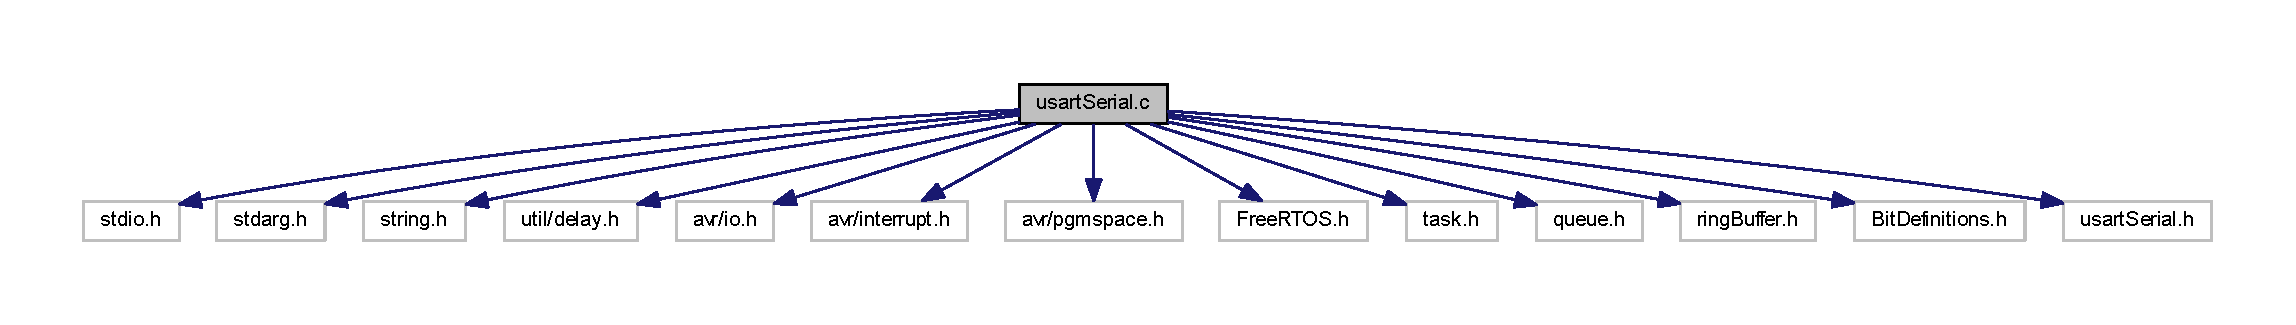
\includegraphics[width=350pt]{usart_serial_8c__incl}
\end{center}
\end{figure}
\subsection*{Data Structures}
\begin{DoxyCompactItemize}
\item 
struct {\bf U\+S\+A\+R\+T\+\_\+\+C\+O\+M\+\_\+\+B\+U\+F}
\begin{DoxyCompactList}\small\item\em Structure of buffers to support communications with a U\+S\+A\+R\+T. \end{DoxyCompactList}\item 
struct {\bf U\+S\+A\+R\+T\+\_\+\+R\+E\+G\+I\+S\+T\+E\+R\+S}
\begin{DoxyCompactList}\small\item\em Structure of pointers to U\+S\+A\+R\+T registers. \end{DoxyCompactList}\end{DoxyCompactItemize}
\subsection*{Macros}
\begin{DoxyCompactItemize}
\item 
\#define {\bfseries R\+X\+C\+\_\+\+B\+I\+T}~B\+I\+T7\label{group__usart_async_module_ga2133aeaf30d1d8f6f819d2252dcdbe8c}

\item 
\#define {\bfseries T\+X\+C\+\_\+\+B\+I\+T}~B\+I\+T6\label{group__usart_async_module_ga6baa91108d3c2d172e44bc70956b98d2}

\item 
\#define {\bfseries U\+D\+R\+E\+\_\+\+B\+I\+T}~B\+I\+T5\label{group__usart_async_module_ga774a9a790e2e547044eddf47e931a1f8}

\item 
\#define {\bfseries F\+E\+\_\+\+B\+I\+T}~B\+I\+T4\label{group__usart_async_module_gaaee51057462df51f411e67a131165914}

\item 
\#define {\bfseries D\+O\+R\+\_\+\+B\+I\+T}~B\+I\+T3\label{group__usart_async_module_ga42bba56b7ce519d770f6791da46b3f64}

\item 
\#define {\bfseries U\+P\+E\+\_\+\+B\+I\+T}~B\+I\+T2\label{group__usart_async_module_gaaa081c9d68175cca9b7a57927616baf1}

\item 
\#define {\bfseries U2\+X\+\_\+\+B\+I\+T}~B\+I\+T1\label{group__usart_async_module_gaffd8feb2e774dd114102f1f8be6599aa}

\item 
\#define {\bfseries R\+X\+C\+I\+E\+\_\+\+B\+I\+T}~B\+I\+T7\label{group__usart_async_module_ga4155881309ac7b270c766149bc9a4bbd}

\item 
\#define {\bfseries U\+D\+R\+I\+E\+\_\+\+B\+I\+T}~B\+I\+T5\label{group__usart_async_module_gaf64c1f6cfda10c415407572973d3f71c}

\item 
\#define {\bfseries R\+X\+E\+N\+\_\+\+B\+I\+T}~B\+I\+T4\label{group__usart_async_module_ga906dab704ddcdb3d2d06384a94126c23}

\item 
\#define {\bfseries T\+X\+E\+N\+\_\+\+B\+I\+T}~B\+I\+T3\label{group__usart_async_module_gae3f799c1bacbb79826d19f6f68c9ddde}

\item 
\#define {\bfseries U\+C\+S\+Z1\+\_\+\+B\+I\+T}~B\+I\+T2\label{group__usart_async_module_ga9f7f7ba3dc9cf8409364251f5167589d}

\item 
\#define {\bfseries U\+C\+S\+Z0\+\_\+\+B\+I\+T}~B\+I\+T1\label{group__usart_async_module_gabc8fadc00f40b4574889185ded4f33f2}

\item 
\#define {\bfseries N\+U\+M\+\_\+\+U\+S\+A\+R\+T\+S}~4\label{group__usart_async_module_ga6829feca87a1bc576152b06505b91617}

\end{DoxyCompactItemize}
\subsection*{Enumerations}
\begin{DoxyCompactItemize}
\item 
enum {\bf U\+S\+A\+R\+T\+\_\+\+S\+T\+A\+T\+E} \{ {\bf V\+A\+C\+A\+N\+T}, 
{\bf E\+N\+G\+A\+G\+E\+D}
 \}
\begin{DoxyCompactList}\small\item\em Defines the state of the U\+S\+A\+R\+T. \end{DoxyCompactList}\end{DoxyCompactItemize}
\subsection*{Functions}
\begin{DoxyCompactItemize}
\item 
int8\+\_\+t {\bf usart\+Check\+Rx\+Complete} (U\+S\+A\+R\+T\+\_\+\+I\+D usart\+Id)
\begin{DoxyCompactList}\small\item\em Check if reception is complete. The function returns the status of the R\+X\+C bit of the U\+S\+A\+R\+T. When set, the bit indicates that data can be read from the U\+S\+A\+R\+T. \end{DoxyCompactList}\item 
int8\+\_\+t {\bf usart\+Check\+Tx\+Ready} (U\+S\+A\+R\+T\+\_\+\+I\+D usart\+Id)
\begin{DoxyCompactList}\small\item\em Check if transmission is complete. The function returns the status of the U\+D\+R\+E bit of the U\+S\+A\+R\+T. When set, the bit indicates that data can be written to the U\+S\+A\+R\+T. \end{DoxyCompactList}\item 
void {\bfseries usart\+\_\+fprintf\+\_\+arg} (U\+S\+A\+R\+T\+\_\+\+I\+D usart\+Id, const char $\ast$format, va\+\_\+list ap)\label{group__usart_async_module_gad3cf1cbb614711dcb8b73f7b7066cc24}

\item 
void {\bfseries usart\+\_\+fprintf\+\_\+\+P\+\_\+arg} (U\+S\+A\+R\+T\+\_\+\+I\+D usart\+Id, P\+G\+M\+\_\+\+P format, va\+\_\+list arg)\label{group__usart_async_module_ga8b9e6d432ec75ce20fd8225d02cd8340}

\item 
void {\bfseries usart\+\_\+xfprintf\+\_\+arg} (U\+S\+A\+R\+T\+\_\+\+I\+D usart\+Id, const char $\ast$format, va\+\_\+list arg)\label{group__usart_async_module_ga7f6efaab6a3c0a43d34bcce2f45a9062}

\item 
void {\bfseries usart\+\_\+xfprintf\+\_\+\+P\+\_\+arg} (U\+S\+A\+R\+T\+\_\+\+I\+D usart\+Id, P\+G\+M\+\_\+\+P format, va\+\_\+list arg)\label{group__usart_async_module_ga33e17cf0120f57e061a736a8eeb93fce}

\item 
void {\bf xmit\+Interrupt\+\_\+\+On} (U\+S\+A\+R\+T\+\_\+\+I\+D)
\item 
void {\bf xmit\+Interrupt\+\_\+\+Off} (U\+S\+A\+R\+T\+\_\+\+I\+D)
\item 
void {\bf usart\+\_\+rx\+\_\+isr} (U\+S\+A\+R\+T\+\_\+\+I\+D)
\item 
void {\bf usart\+\_\+tx\+\_\+isr} (U\+S\+A\+R\+T\+\_\+\+I\+D)
\item 
U\+S\+A\+R\+T\+\_\+\+I\+D {\bf usart\+Open} (U\+S\+A\+R\+T\+\_\+\+I\+D usart\+Id, uint32\+\_\+t ul\+Wanted\+Baud, uint16\+\_\+t ux\+Tx\+Queue\+Length, uint16\+\_\+t ux\+Rx\+Queue\+Length)
\begin{DoxyCompactList}\small\item\em Open a connection on a U\+S\+A\+R\+T. \end{DoxyCompactList}\item 
void {\bf set\+Default\+U\+S\+A\+R\+T} (U\+S\+A\+R\+T\+\_\+\+I\+D usart\+Id)
\begin{DoxyCompactList}\small\item\em Update default U\+S\+A\+R\+T. \end{DoxyCompactList}\item 
void {\bf usart\+Close} (U\+S\+A\+R\+T\+\_\+\+I\+D usart\+Id)
\begin{DoxyCompactList}\small\item\em Close a connection on a U\+S\+A\+R\+T. \end{DoxyCompactList}\item 
void {\bf usart\+\_\+printf} (const char $\ast$format,...)
\begin{DoxyCompactList}\small\item\em Standard printf function. \end{DoxyCompactList}\item 
void {\bf usart\+\_\+printf\+\_\+\+P} (P\+G\+M\+\_\+\+P format,...)
\begin{DoxyCompactList}\small\item\em Standard printf function that uses a formating string stored in memory. \end{DoxyCompactList}\item 
void {\bf usart\+\_\+print} (uint8\+\_\+t $\ast$str)
\begin{DoxyCompactList}\small\item\em Print string on default U\+S\+A\+R\+T. \end{DoxyCompactList}\item 
void {\bf usart\+\_\+print\+\_\+\+P} (P\+G\+M\+\_\+\+P str)
\begin{DoxyCompactList}\small\item\em Print string stored in program memory on default U\+S\+A\+R\+T. \end{DoxyCompactList}\item 
void {\bf usart\+\_\+fprintf} (int usartid, const char $\ast$format,...)
\begin{DoxyCompactList}\small\item\em Standard printf for specified U\+S\+A\+R\+T. \end{DoxyCompactList}\item 
void {\bf usart\+\_\+fprintf\+\_\+\+P} (int usart\+Id, P\+G\+M\+\_\+\+P format,...)
\begin{DoxyCompactList}\small\item\em Standard printf function for specific U\+S\+A\+R\+T with formating string in program memory. \end{DoxyCompactList}\item 
void {\bf usart\+\_\+fprint} (U\+S\+A\+R\+T\+\_\+\+I\+D usart\+Id, uint8\+\_\+t $\ast$str)
\begin{DoxyCompactList}\small\item\em Print string to specific U\+S\+A\+R\+T. \end{DoxyCompactList}\item 
void {\bf usart\+\_\+fprint\+\_\+\+P} (U\+S\+A\+R\+T\+\_\+\+I\+D usart\+Id, P\+G\+M\+\_\+\+P str)
\begin{DoxyCompactList}\small\item\em Print a string stored in program memory to specific U\+S\+A\+R\+T. \end{DoxyCompactList}\item 
void {\bf usart\+Write} (U\+S\+A\+R\+T\+\_\+\+I\+D usart\+Id, int8\+\_\+t data\+Out)
\begin{DoxyCompactList}\small\item\em Low level write function (single character). Will delay until usart is ready to accept the 8 bit data. \end{DoxyCompactList}\item 
int8\+\_\+t {\bf usart\+Read} (U\+S\+A\+R\+T\+\_\+\+I\+D usart\+Id)
\begin{DoxyCompactList}\small\item\em Low level read function (single character). Delays until data available from the U\+S\+A\+R\+T. Will check for reception errors. \end{DoxyCompactList}\item 
void {\bf usart\+\_\+xprintf} (const char $\ast$format,...)
\begin{DoxyCompactList}\small\item\em Standard printf (interrupt driven) to default U\+S\+A\+R\+T. \end{DoxyCompactList}\item 
void {\bf usart\+\_\+xprintf\+\_\+\+P} (P\+G\+M\+\_\+\+P format,...)
\begin{DoxyCompactList}\small\item\em Standard printf (interrupt driven) to default U\+S\+A\+R\+T using formating string stored in program memory. \end{DoxyCompactList}\item 
void {\bf usart\+\_\+xprint} (uint8\+\_\+t $\ast$str)
\begin{DoxyCompactList}\small\item\em Prints a string on the default U\+S\+A\+R\+T (defined by default\+U\+S\+A\+R\+T). \end{DoxyCompactList}\item 
void {\bf usart\+\_\+xprint\+\_\+\+P} (P\+G\+M\+\_\+\+P str)
\begin{DoxyCompactList}\small\item\em Prints a string stored in program memory on the default U\+S\+A\+R\+T (defined by default\+U\+S\+A\+R\+T). \end{DoxyCompactList}\item 
void {\bf usart\+\_\+xfprintf} (int usart\+Id, const char $\ast$format,...)
\begin{DoxyCompactList}\small\item\em Standard printf function for specific U\+S\+A\+R\+T. \end{DoxyCompactList}\item 
void {\bf usart\+\_\+xfprintf\+\_\+\+P} (int usart\+Id, P\+G\+M\+\_\+\+P format,...)
\begin{DoxyCompactList}\small\item\em Standard printf function for specific U\+S\+A\+R\+T that uses a formating string stored in program memory. \end{DoxyCompactList}\item 
void {\bf usart\+\_\+xfprint} (U\+S\+A\+R\+T\+\_\+\+I\+D usart\+Id, uint8\+\_\+t $\ast$str)
\begin{DoxyCompactList}\small\item\em Print string to specific U\+S\+A\+R\+T. \end{DoxyCompactList}\item 
void {\bf usart\+\_\+xfprint\+\_\+\+P} (U\+S\+A\+R\+T\+\_\+\+I\+D usart\+Id, P\+G\+M\+\_\+\+P str)
\begin{DoxyCompactList}\small\item\em Print string stored in program memory to specific U\+S\+A\+R\+T. \end{DoxyCompactList}\item 
void {\bf usart\+\_\+xflush\+Rx} (U\+S\+A\+R\+T\+\_\+\+I\+D usart\+Id)
\begin{DoxyCompactList}\small\item\em Flushes all characters in the receive ring buffer (i.\+e. empties the buffer). \end{DoxyCompactList}\item 
uint16\+\_\+t {\bf usart\+\_\+\+Available\+Char\+Rx} (U\+S\+A\+R\+T\+\_\+\+I\+D usart\+Id)
\begin{DoxyCompactList}\small\item\em Gives number of bytes in reception ring buffer. \end{DoxyCompactList}\item 
U\+Base\+Type\+\_\+t {\bf usart\+\_\+xget\+Char} (U\+S\+A\+R\+T\+\_\+\+I\+D usart\+Id, U\+Base\+Type\+\_\+t $\ast$pc\+Rxed\+Char)
\begin{DoxyCompactList}\small\item\em Get a character from the reception ring buffer. \end{DoxyCompactList}\item 
U\+Base\+Type\+\_\+t {\bf usart\+\_\+xput\+Char} (U\+S\+A\+R\+T\+\_\+\+I\+D usart\+Id, const U\+Base\+Type\+\_\+t c\+Out\+Char)
\begin{DoxyCompactList}\small\item\em Drops a character into the transmit ring buffer. \end{DoxyCompactList}\item 
{\bfseries I\+S\+R} (U\+S\+A\+R\+T0\+\_\+\+R\+X\+\_\+vect)\label{group__usart_async_module_ga084f0a9cf05b1877bd8a71a90dae7ff8}

\item 
{\bfseries I\+S\+R} (U\+S\+A\+R\+T1\+\_\+\+R\+X\+\_\+vect)\label{group__usart_async_module_gae6e8a8009a9ae0c59f25a496d1cf5a84}

\item 
{\bfseries I\+S\+R} (U\+S\+A\+R\+T2\+\_\+\+R\+X\+\_\+vect)\label{group__usart_async_module_ga63a86aad9ba2e355fe6380da553f554e}

\item 
{\bfseries I\+S\+R} (U\+S\+A\+R\+T3\+\_\+\+R\+X\+\_\+vect)\label{group__usart_async_module_ga88e32db0cad75219c51253f5c1052fc0}

\item 
{\bfseries I\+S\+R} (U\+S\+A\+R\+T0\+\_\+\+U\+D\+R\+E\+\_\+vect)\label{group__usart_async_module_ga95e67e677722a53e3ad9f1ffce2e7408}

\item 
{\bfseries I\+S\+R} (U\+S\+A\+R\+T1\+\_\+\+U\+D\+R\+E\+\_\+vect)\label{group__usart_async_module_gad6441110baf548d12ae53fcbed8075c5}

\item 
{\bfseries I\+S\+R} (U\+S\+A\+R\+T2\+\_\+\+U\+D\+R\+E\+\_\+vect)\label{group__usart_async_module_ga6dd0f9b7dad929f4170efd85c67e04ba}

\item 
{\bfseries I\+S\+R} (U\+S\+A\+R\+T3\+\_\+\+U\+D\+R\+E\+\_\+vect)\label{group__usart_async_module_ga965b31b0729ebabd50c26e4557d9609d}

\end{DoxyCompactItemize}
\subsection*{Variables}
\begin{DoxyCompactItemize}
\item 
{\bf U\+S\+A\+R\+T\+\_\+\+R\+E\+G\+I\+S\+T\+E\+R\+S} {\bf usart\+Reg} [$\,$]
\item 
{\bf U\+S\+A\+R\+T\+\_\+\+C\+O\+M\+\_\+\+B\+U\+F} {\bf usart\+Com\+Buf} [N\+U\+M\+\_\+\+U\+S\+A\+R\+T\+S]
\item 
U\+S\+A\+R\+T\+\_\+\+I\+D {\bf default\+U\+S\+A\+R\+T} = U\+S\+A\+R\+T0
\end{DoxyCompactItemize}


\subsection{Detailed Description}
Module for asynchronous communication with the Atmega2560 U\+S\+A\+R\+T\textquotesingle{}s. 

\begin{DoxyAuthor}{Author}
Gilbert Arbez 
\end{DoxyAuthor}
\begin{DoxyDate}{Date}
May 26 2015 Both interrupt driven and polling functions are available.
\end{DoxyDate}
Uses free\+R\+T\+O\+S ring buffers to support interrupt functions. 
%--- End generated contents ---

% Index
\backmatter
\newpage
\phantomsection
\clearemptydoublepage
\addcontentsline{toc}{chapter}{Index}
\printindex

\end{document}
